% Options for packages loaded elsewhere
\PassOptionsToPackage{unicode}{hyperref}
\PassOptionsToPackage{hyphens}{url}
%
\documentclass[
  english,
  man,floatsintext]{apa6}
\usepackage{amsmath,amssymb}
\usepackage{lmodern}
\usepackage{ifxetex,ifluatex}
\ifnum 0\ifxetex 1\fi\ifluatex 1\fi=0 % if pdftex
  \usepackage[T1]{fontenc}
  \usepackage[utf8]{inputenc}
  \usepackage{textcomp} % provide euro and other symbols
\else % if luatex or xetex
  \usepackage{unicode-math}
  \defaultfontfeatures{Scale=MatchLowercase}
  \defaultfontfeatures[\rmfamily]{Ligatures=TeX,Scale=1}
\fi
% Use upquote if available, for straight quotes in verbatim environments
\IfFileExists{upquote.sty}{\usepackage{upquote}}{}
\IfFileExists{microtype.sty}{% use microtype if available
  \usepackage[]{microtype}
  \UseMicrotypeSet[protrusion]{basicmath} % disable protrusion for tt fonts
}{}
\makeatletter
\@ifundefined{KOMAClassName}{% if non-KOMA class
  \IfFileExists{parskip.sty}{%
    \usepackage{parskip}
  }{% else
    \setlength{\parindent}{0pt}
    \setlength{\parskip}{6pt plus 2pt minus 1pt}}
}{% if KOMA class
  \KOMAoptions{parskip=half}}
\makeatother
\usepackage{xcolor}
\IfFileExists{xurl.sty}{\usepackage{xurl}}{} % add URL line breaks if available
\IfFileExists{bookmark.sty}{\usepackage{bookmark}}{\usepackage{hyperref}}
\hypersetup{
  pdftitle={Exploring reliability heterogeneity with multiverse analyses: Data processing decisions unpredictably influence measurement reliability},
  pdfauthor={Sam Parsons1},
  pdflang={en-EN},
  pdfkeywords={reliability, multiverse, analytic flexibility, data processing},
  hidelinks,
  pdfcreator={LaTeX via pandoc}}
\urlstyle{same} % disable monospaced font for URLs
\usepackage{graphicx}
\makeatletter
\def\maxwidth{\ifdim\Gin@nat@width>\linewidth\linewidth\else\Gin@nat@width\fi}
\def\maxheight{\ifdim\Gin@nat@height>\textheight\textheight\else\Gin@nat@height\fi}
\makeatother
% Scale images if necessary, so that they will not overflow the page
% margins by default, and it is still possible to overwrite the defaults
% using explicit options in \includegraphics[width, height, ...]{}
\setkeys{Gin}{width=\maxwidth,height=\maxheight,keepaspectratio}
% Set default figure placement to htbp
\makeatletter
\def\fps@figure{htbp}
\makeatother
\setlength{\emergencystretch}{3em} % prevent overfull lines
\providecommand{\tightlist}{%
  \setlength{\itemsep}{0pt}\setlength{\parskip}{0pt}}
\setcounter{secnumdepth}{-\maxdimen} % remove section numbering
% Make \paragraph and \subparagraph free-standing
\ifx\paragraph\undefined\else
  \let\oldparagraph\paragraph
  \renewcommand{\paragraph}[1]{\oldparagraph{#1}\mbox{}}
\fi
\ifx\subparagraph\undefined\else
  \let\oldsubparagraph\subparagraph
  \renewcommand{\subparagraph}[1]{\oldsubparagraph{#1}\mbox{}}
\fi
% Manuscript styling
\usepackage{upgreek}
\captionsetup{font=singlespacing,justification=justified}

% Table formatting
\usepackage{longtable}
\usepackage{lscape}
% \usepackage[counterclockwise]{rotating}   % Landscape page setup for large tables
\usepackage{multirow}		% Table styling
\usepackage{tabularx}		% Control Column width
\usepackage[flushleft]{threeparttable}	% Allows for three part tables with a specified notes section
\usepackage{threeparttablex}            % Lets threeparttable work with longtable

% Create new environments so endfloat can handle them
% \newenvironment{ltable}
%   {\begin{landscape}\centering\begin{threeparttable}}
%   {\end{threeparttable}\end{landscape}}
\newenvironment{lltable}{\begin{landscape}\centering\begin{ThreePartTable}}{\end{ThreePartTable}\end{landscape}}

% Enables adjusting longtable caption width to table width
% Solution found at http://golatex.de/longtable-mit-caption-so-breit-wie-die-tabelle-t15767.html
\makeatletter
\newcommand\LastLTentrywidth{1em}
\newlength\longtablewidth
\setlength{\longtablewidth}{1in}
\newcommand{\getlongtablewidth}{\begingroup \ifcsname LT@\roman{LT@tables}\endcsname \global\longtablewidth=0pt \renewcommand{\LT@entry}[2]{\global\advance\longtablewidth by ##2\relax\gdef\LastLTentrywidth{##2}}\@nameuse{LT@\roman{LT@tables}} \fi \endgroup}

% \setlength{\parindent}{0.5in}
% \setlength{\parskip}{0pt plus 0pt minus 0pt}

% \usepackage{etoolbox}
\makeatletter
\patchcmd{\HyOrg@maketitle}
  {\section{\normalfont\normalsize\abstractname}}
  {\section*{\normalfont\normalsize\abstractname}}
  {}{\typeout{Failed to patch abstract.}}
\patchcmd{\HyOrg@maketitle}
  {\section{\protect\normalfont{\@title}}}
  {\section*{\protect\normalfont{\@title}}}
  {}{\typeout{Failed to patch title.}}
\makeatother
\shorttitle{Reliability multiverse}
\keywords{reliability, multiverse, analytic flexibility, data processing}
\usepackage{csquotes}
\usepackage{float}
\usepackage{caption}
\usepackage{newunicodechar}
\floatplacement{figure}{H}
\raggedbottom
\ifxetex
  % Load polyglossia as late as possible: uses bidi with RTL langages (e.g. Hebrew, Arabic)
  \usepackage{polyglossia}
  \setmainlanguage[]{english}
\else
  \usepackage[main=english]{babel}
% get rid of language-specific shorthands (see #6817):
\let\LanguageShortHands\languageshorthands
\def\languageshorthands#1{}
\fi
\ifluatex
  \usepackage{selnolig}  % disable illegal ligatures
\fi
\newlength{\cslhangindent}
\setlength{\cslhangindent}{1.5em}
\newlength{\csllabelwidth}
\setlength{\csllabelwidth}{3em}
\newenvironment{CSLReferences}[2] % #1 hanging-ident, #2 entry spacing
 {% don't indent paragraphs
  \setlength{\parindent}{0pt}
  % turn on hanging indent if param 1 is 1
  \ifodd #1 \everypar{\setlength{\hangindent}{\cslhangindent}}\ignorespaces\fi
  % set entry spacing
  \ifnum #2 > 0
  \setlength{\parskip}{#2\baselineskip}
  \fi
 }%
 {}
\usepackage{calc}
\newcommand{\CSLBlock}[1]{#1\hfill\break}
\newcommand{\CSLLeftMargin}[1]{\parbox[t]{\csllabelwidth}{#1}}
\newcommand{\CSLRightInline}[1]{\parbox[t]{\linewidth - \csllabelwidth}{#1}\break}
\newcommand{\CSLIndent}[1]{\hspace{\cslhangindent}#1}

\title{Exploring reliability heterogeneity with multiverse analyses: Data processing decisions unpredictably influence measurement reliability}
\author{Sam Parsons\textsuperscript{1}}
\date{}


\authornote{

Submitted to Meta-Psychology. Click here to follow the fully transparent editorial process of this submission. Participate in open peer review by commenting through hypothes.is directly on this preprint.

Sam Parsons is currently supported by a Radboud Excellence Fellowship. This work was initually supported by an ESRC grant {[}ES/R004285/1{]}

I would like to thank Ana Todorovic for her insightful feedback on an earlier version of this manuscript.

Correspondence concerning this article should be addressed to Sam Parsons, Cognitive Neuroscience Department, Donders Institute for Brain, Cognition and Behavior, Radboud University Medical Center, Nijmegen, the Netherlands. E-mail: \href{mailto:sam.parsons@radboudumc.nl}{\nolinkurl{sam.parsons@radboudumc.nl}}

}

\affiliation{\vspace{0.5cm}\textsuperscript{1} Radboud University Medical Center}

\abstract{
Analytic flexibility is known to influence the results of statistical tests, e.g.~effect sizes and p-values. Yet, the degree to which flexibility in data processing decisions influences measurement reliability is unknown. In this paper I attempt to address this question using a series of 36 reliability multiverse analyses, each with 288 data processing specifications, including accuracy and response time cut-offs. I used data from a Stroop task and Flanker task at two time points, as well as a Dot Probe task across three stimuli conditions and three timepoints. This allowed for broad overview of internal consistency reliability and test-retest estimates across a multiverse of data processing specifications. Largely arbitrary decisions in data processing led to differences between the highest and lowest reliability estimate of at least 0.2, but potentially exceeding 0.7. Importantly, there was no consistent pattern in reliability estimates resulting from the data processing specifications, across time as well as tasks. Together, data processing decisions are highly influential, and largely unpredictable, on measure reliability. I discuss actions researchers could take to mitigate some of the influence of reliability heterogeneity, including adopting hierarchical modelling approaches. Yet, there are no approaches that can completely save us from measurement error. Measurement matters and I call on readers to help us move from what could be a measurement crisis towards a measurement revolution.
}



\begin{document}
\maketitle

In this paper I was concerned with the influence analytic flexibility on measurement reliability, specifically in data processing or data cleaning. I took inspiration from numerous papers reporting the unsettlingly low reliability of Dot Probe attention bias indices (e.g. Jones, Christiansen, \& Field, 2018; Schmukle, 2005; Staugaard, 2009) and other work investigating alternative analyses and data processing strategies, with the intention of yielding a more reliable measurement (e.g. Jones, Christiansen, \& Field, 2018; Price et al., 2015). When considering the impact of researcher degrees of freedom, focus is drawn to decisions made in the beginning (task design) or at the end (data analysis) of the research process. I was interested in the middle step: data processing and measure reliability. In this paper, I explore and visualise the influence of data processing steps on reliability using a series of reliability multiverse analyses.

\hypertarget{getting-up-to-speed-with-reliability}{%
\subsection{Getting up to speed with reliability}\label{getting-up-to-speed-with-reliability}}

The accuracy of our conclusions rests on the quality, and the strength, of our evidence. Our evidence rests on the bedrock of our measurements. The quality of our measures defines the quality of our results. Without adequate focus on the validity of our measures, how can we be assured that we are capturing the concept or process that we are interested in? Without any attention to the reliability of our measures, how can we be sure that we are capturing a phenomenon with any precision? Psychological science has a guilty habit of neglecting these foundations, though of course some areas fair better than others.

In a recent paper, my colleagues and I argued for a widespread appreciation for the reliability of our cognitive measures (Parsons, Kruijt, \& Fox, 2019). Briefly, low reliability places doubt on the veracity of statistical analyses using that measure; measurement reliability restricts the observable range of effect sizes in simple correlational analyses, and unpredictably in more complicated models; and failing to correct for measurement error makes comparing effect sizes between, and within, studies difficult. These issues are compounded by the sad observation that the reporting of reliability (and validity) evidence is woefully poor. Scale validity and reliability is not routinely examined, and many scales are adapted on an ad hoc basis with little or no validation (Flake, Pek, \& Hehman, 2017). In other cases scales fail to pass deeper psychometric evaluation, including tests of measurement invariance (Hussey \& Hughes, 2018). This likely reflects issues with more superficial approaches to establishing validity evidence - i.e.~reporting Cronbach's alpha, stating it is adequate, and moving on. Pockets of psychological science take a more enlightened approach. However, I feel it is reasonable to argue that the field at large is not doing well in our measurement practices. Most relevant to this paper; it is the exception rather than the norm to evaluate the psychometric properties of cognitive measurements (Gawronski, Deutsch, \& Banse, 2011).

Strictly speaking, we cannot state that a task is unreliable; although we might observe a consistent pattern of unreliability in measurements obtained that causes us to question further use of the task. An important reminder: estimates of reliability refer to the measurement obtained - in a specific sample and under particular circumstances, including the task parameters. Reliability is therefore not fixed; it may differ between populations, samples, and testing conditions. Variations of a task may lead to the generation of more or less reliable measurements. For example, the stimulus presentation duration will likely influence the cognitive processes involved in completing the task, perhaps leading participants to perform more consistently in one version, relative to another. Reliability is a property of the measurement, not of the task used to obtain it. In this study, we are concerned with the data processing steps researchers take and how these influence our measurement, and the resulting reliability estimates. To explore this, I invite you to join me, dear reader, on a walk through the garden of forking paths.

\hypertarget{analytic-flexibility-and-the-garden-of-forking-paths}{%
\subsection{Analytic flexibility and the garden of forking paths}\label{analytic-flexibility-and-the-garden-of-forking-paths}}

Every result presented in every research article is the culmination of many decisions made by one or more researchers; the sheer number of combinations of valid decisions is likely uncalculatable. The ``garden of forking paths'' (Gelman \& Loken, 2013) is a useful analogy to illustrate this. With each decision that must be made, however arbitrary, the researcher comes to a fork in their research path and selects one. To add a little suspense, there will be many cases when the researcher does not notice a fork in the road. Perhaps the researcher unconsciously makes the same turn as always, their feet working of their own accord. These forks in the path, the decisions researchers make (whether they are aware or not), may be reasonably combined to make a near uncountable number of paths. Each path also leads to a location; some paths end close to one another, and other times the paths diverge wildly. We can think of the end of the path as the statistical result our researcher arrives at.

The researcher has to decide their path, based on the soundest justifications they can make at each fork (e.g. Lakens et al., 2018). Of course, psychological science has become fully aware of the detrimental effects of selecting one's path retrospectively, based on where the path ends or the results most exciting to the researcher (read as: \emph{p} \textless{} .05; e.g. Simmons, Nelson, \& Simonsohn, 2011). Analytic flexibility is not inherently bad. However, we must acknowledge the ramifications. The effects we observe, or do not, are potentially influenced by all of the decisions made to arrive at them. Thus, a range of possible effects may have been observed that could be more or less equally valid or justifiable based on the analytical decisions made.

In discussions of analytical flexibility, focus is usually given primarily to decisions made during statistical analysis. For example, should I control for age and gender? Do I reason that this is model more appropriate over that one? Or where should I set my alpha and how should I justify the decision? Discussions of analytical flexibility often concern issues around \emph{p}-hacking and other QRPs (intended or unintended). However, as Leek and Peng (2015) note, \emph{p}-values are the tip of the iceberg; not enough scrutiny is given to the impact of the many steps in the research pipeline that precede inference testing. I agree. In my estimation, flexibility in measurement and data handling do not receive the scrutiny they deserve. If the garden of forking paths concerns analytic flexibility, then measurement flexibility decides which gateway one enters the garden through in the first place. As an example, a recent review highlighted the lack of consensus around the processing of task data from tasks in the attention control literature, including but not limited to the data pre-processing used in this paper (Bastian et al., 2020, pp. 47--48)

\hypertarget{mapping-the-garden-of-forking-paths-with-multiverse-analyses}{%
\subsection{Mapping the garden of forking paths with multiverse analyses}\label{mapping-the-garden-of-forking-paths-with-multiverse-analyses}}

Multiverse analyses (Steegen, Tuerlinckx, Gelman, \& Vanpaemel, 2016) offers us a ``GPS in the garden of forking paths'' (Quintana \& Heathers, 2019). The process is simpler than one might expect. First, we define a set of reasonable data processing and analysis decisions. Second, we run the entire set of analyses. We can then examine results across the entire range of results. Specification curve analysis (Simonsohn, Simmons, \& Nelson, 2015) adds third step allowing for inference tests across the distribution of results generated in the multiverse (for insightful applications of specification curve analyses, see Orben \& Przybylski, 2019; Rohrer, Egloff, \& Schmukle, 2017). In this paper I use `specification' to refer to each combination of data processing decisions in the multiverse analysis.

Multiverse analyses enable us to explore how a researcher's -- sometimes arbitrary -- choices in data processing (e.g.~outlier removal) and analysis decisions (e.g.~including covariates, splitting samples) influence statistical results, and the conclusions drawn from the analysis. From this we can examine which choices are more or less influential than others, as well as how robust the result is across the full set of specifications.

\hypertarget{a-reliability-multiverse-from-many-data-processing-decisions}{%
\subsection{A reliability multiverse from many data processing decisions}\label{a-reliability-multiverse-from-many-data-processing-decisions}}

In this paper I report multiverse analyses exploring the influence of data processing specifications on the reliability of a calculated measurement. I used openly accessible Stroop task and Flanker task data generously shared by Hedge and colleagues (Hedge, Powell, \& Sumner, 2018) and Dot Probe task data from the CogBIAS project (Booth, Songco, Parsons, Heathcote, \& Fox, 2019; Booth et al., 2017). Following our previous work in this area (Parsons, Kruijt, \& Fox, 2019), I was interested in the stability and range of reliability estimates on cognitive-behavioural measures. Broadly, I was interested in the impact of data processing decisions on reliability. It is possible that certain analytic decisions tend to yield higher reliability estimates; it may be that particular combinations of decisions are also better, or worse, than others. Beyond that, I was interested in the range of estimates. A small range would suggest that measure reliability is relatively stable as we make potentially arbitrary data processing decisions while walking the garden of forking paths. A large range suggests hidden measurement reliability heterogeneity. This is potentially an important, and underappreciated, contributor to the replicability crisis (Loken \& Gelman, 2017). Alternatively, this could be a herald for a crisis of measurement.

\hypertarget{methods}{%
\section{Methods}\label{methods}}

\hypertarget{data}{%
\subsection{Data}\label{data}}

Stroop and Flanker task data were obtained from the online repository for Hedge, Sumner, and Powell (2018, \url{https://osf.io/cwzds/}). Full details of the data collection, study design, and procedure can be found in Hedge et al. (2018). These data are ideal for our purposes as they a) contain many trials, helping us obtain more precise estimates of reliability, and b) include two assessment time-points approximately 3-4 weeks apart, allowing us to explore both: internal consistency and test-retest reliability. The data were collected from different studies; for simplicity in this paper, the data across studies were pooled (n = 107 before any data processing -- note that this may be different from the sample size presented by Hedge et al.~due to differences in data processing).

Dot Probe data were obtained from the CogBIAS project (Booth, Songco, Parsons, Heathcote, \& Fox, 2019; Booth et al., 2017). Full details of the full study and data collection can be found in Booth et al.~(2017, 2019). These data complement the Stroop and Flanker data as they provide a longer test-retest duration (approximately 1.5 years between repeated measures) across three timepoints. In addition, the task incorporated three stimuli conditions, allowing us cross-sectional comparisons of reliability stability within the same task. The Dot Probe data were pooled such that only a subset of participants completing the task at all three timepoints were retained (n = 285).

Interested readers can find the data and code used to perform the multiverse analyses and generate this manuscript in the Open Science Framework repository for this project (\url{https://osf.io/haz6u/}).\footnote{I used the following R packages for all analyses and figures, and to generate this document: R {[}Version 4.1.0; R Core Team (2018){]} and the R-packages \emph{Cairo} {[}Version 1.5.12.2; Urbanek and Horner (2019){]}, \emph{dplyr} {[}Version 1.0.7; Wickham, François, Henry, and Müller (2019){]}, \emph{forcats} {[}Version 0.5.1; Wickham (2019a){]}, \emph{ggplot2} {[}Version 3.3.5; Wickham (2016){]}, \emph{gridExtra} {[}Version 2.3; Auguie (2017){]}, \emph{papaja} {[}Version 0.1.0.9997; Aust and Barth (2018){]}, \emph{patchwork} {[}Version 1.1.1; Pedersen (2019){]}, \emph{psych} {[}Version 2.1.6; Revelle (2019){]}, \emph{purrr} {[}Version 0.3.4; Henry and Wickham (2019){]}, \emph{readr} {[}Version 1.4.0; Wickham, Hester, and Francois (2018){]}, \emph{splithalf} {[}Version 0.8.1; Parsons (2019){]}, \emph{stringr} {[}Version 1.4.0; Wickham (2019b){]}, \emph{tibble} {[}Version 3.1.6; Müller and Wickham (2019){]}, \emph{tidyr} {[}Version 1.1.3; Wickham and Henry (2019){]}, and \emph{tidyverse} {[}Version 1.3.1; Wickham et al. (2019){]}}

\hypertarget{stroop-task}{%
\subsubsection{Stroop task}\label{stroop-task}}

Participants made keyed responses to the colour of a word presented in the centre of the screen. In congruent conditions the word was the same as the font colour, whereas, in incongruent trials, the word was a different colour from the font colour. In a neutral condition, the word was not a colour word. Participants completed 240 of each trial type. The outcome index we explore here is the RT cost, calculated as the average RT for incongruent trials minus the average RT for congruent trials.

\hypertarget{flanker-task}{%
\subsubsection{Flanker task}\label{flanker-task}}

Participants made keyed responses to the colour of a word presented in the centre of the screen. In congruent conditions the word was the same as the font colour, whereas, in incongruent trials, the word was a different colour from the font colour. In a neutral condition, the word was not a colour word. Participants completed 240 of each trial type. The outcome index we explore here is the RT cost, calculated as the average RT for incongruent trials minus the average RT for congruent trials.

\hypertarget{dot-probe-task}{%
\subsubsection{Dot Probe Task}\label{dot-probe-task}}

Participants made keyed responses to the identity of a probe presented on screen. The probe was presented in the same location as one of the paired faces presented on screen for 500ms prior. The paired faces were an emotional face (angry, pained, and happy) paired with a neutral face (taken from the STOIC faces database, Roy et al., 2009). In congruent trials, the probe was presented in the same location as the emotional face. In incongruent trials, the probe was presented in the same location as the neutral face. Participants completed three blocks of 56 trials corresponding to the emotion presented. The `attention bias' outcome index (MacLeod, Mathews, \& Tata, 1986) was calculated as calculated as the average RT for incongruent trials minus the average RT for congruent trials.

\hypertarget{multiverse-analysis}{%
\subsection{Multiverse analysis}\label{multiverse-analysis}}

In a personal effort to make my research reproducible, and also help others perform similar processes I have developed simple functions to perform the multiverse analyses reported in this paper. Readers interested in performing similar analyses can find these functions within the splithalf package (Parsons, 2021) and tutorials on the related GitHub page (\url{https://github.com/sdparsons/splithalf}). The key functions are: \emph{splithalf.multiverse}, \emph{testretest.multiverse}, and \emph{multiverse.plot}. Intraclass Correlation Coefficients (ICC2) were estimated using the psych R package (Revelle, 2019). Interested readers can also inspect the code used to perform the analyses in this paper (\url{https://osf.io/haz6u/}).

\hypertarget{step-1.-creating-a-list-of-all-specifications}{%
\subsubsection{Step 1. Creating a list of all specifications}\label{step-1.-creating-a-list-of-all-specifications}}

No data were removed before the multiverse analysis. To my knowledge, there are no fixed standards in the literature for processing data from any of the tasks. I identified six decisions common to processing RT data, though there are many more. For simplicity I stuck to RT difference scores as the outcome measure of interest. However, there are very different analytical techniques that might be applied to RT tasks such as this (for example, multilevel modelling and drift-diffusion modelling approaches). The decisions were as follows:

\begin{itemize}
\item
  \emph{Total accuracy.} Researchers may opt to remove participants with accuracy lower than a pre-specified cut-off; for example 80 of 90 per cent. I used three options; 80\%, 90\%, and no cut-off.
\item
  \emph{Absolute response time removals.} Researchers will often remove trials faster than a minimum RT threshold and trials that exceed a maximum RT threshold. I use minimum RT cut-offs at 100ms, 200ms, as well as no cut-off. And, I use two maximum RT cutoffs; 3000ms, and 2000ms.
\item
  \emph{Relative RT cut offs.} After absolute RT cut-offs, researchers can decide to remove trials with RTs greater than a number of standard deviations from the mean (sometimes called relative cut-offs or trimmed means). Three SDs from the mean would remove very extreme outliers; two SDs from the mean is common. I have not seen researchers use one SD from the mean as a cut off, as it is likely a too conservative threshold. As I was interested in a wide range of possible specifications, I included one standard deviation. I use no relative cut off, and one, two, and three SDs from the mean cutoffs in the multiverse.
\item
  \emph{Where to apply the relative cutoff.} The decision to remove trials based on a SD cutoff comes with its own decision. Namely, at what granularity? We could remove trials with RTs greater than 2SDs from the participant's average RT, for example. We could also remove trials with RTs greater than 2SDs from the mean RT within each trial type (congruent and incongruent, for example). I included both options; participant level, and trial type level.
\item
  \emph{Averaging.} Most often the mean RT within each trial type is calculated, and may then be analysed directly, or a difference score calculated to analyse. Researchers may opt to use the median RT instead. I included both options.
\end{itemize}

The number of possible combinations (data processing specifications) quickly increases with every additional option. Here we have 3 \(\times\) 2 \(\times\) 3 \(\times\) 4 \(\times\) 2 \(\times\) 2 = 288 possible specifications.

\hypertarget{step-2.-run-all-specifications-and-extract-reliability-estimates}{%
\subsubsection{Step 2. Run all specifications and extract reliability estimates}\label{step-2.-run-all-specifications-and-extract-reliability-estimates}}

From this decision list, we have a complete list of 288 data processing specifications. In the multiverse analysis the data is processed following each specification parameters, before estimating the reliability of the resulting outcome measure. Internal consistency was estimated using 500 permutations of the splithalf (Parsons, 2021) procedure for each specification (5000 is standard, but 500 was selected to reduce processing time). Following Hedge et al.~(2018), and because ICC relates to both the correlation and the agreement among repeated measures, test-retest reliability was estimated using ICC2k (Koo \& Li, 2016).

\hypertarget{step-3.-visualising-the-multiverse}{%
\subsubsection{Step 3. Visualising the multiverse}\label{step-3.-visualising-the-multiverse}}

I find that one of the joys of multiverse analyses are the visualisations, because sometimes science is more art than science. I explain the visualisations in the results section.

\hypertarget{analysis-plan}{%
\subsection{Analysis plan}\label{analysis-plan}}

For the core analysis I performed 18 multiverse analyses following the steps described above. Separately for each of the Stroop and Flanker task data, I examined internal consistency reliability at time 1 and at time 2, as well as test-retest reliability from time 1 to time 2. For the Dot Probe data, I examined internal consistency reliability at each of the three timepoints, separately for the three task conditions, as well as test-retest reliability at across timepoints. For each multiverse I report the median estimate and it's 95\% Confidence Interval, the proportion of estimates exceeding 0.7, and the range of estimates in that multiverse. In addition to visualising each multiverse, I also include visualisations overlapping the internal consistency multiverses over time. These overlapped plots allow us to visually inspect whether the pattern of reliability estimates following the full range of data processing specifications are comparable across each time point.

\hypertarget{inferences-from-the-multiverse}{%
\subsubsection{Inferences from the multiverse}\label{inferences-from-the-multiverse}}

It is not my aim in this paper to make inferences from these reliability multiverse analyses as one would in a specification curve analysis (Simonsohn, Simmons, \& Nelson, 2015). One could use this method to perform inference testing against the curve of reliability estimates. However, it is not clear what this would add: testing whether the reliability estimates significantly differ from zero is a low bar for assessing the reliability of a measure.

\hypertarget{results}{%
\section{Results}\label{results}}

I include a visualisation for each multiverse analysis. The reliability estimates are presented on the y-axis at the top of the figure; each estimate is represented by a black dot and the 95\% confidence interval is represented by the shaded band. The x-axis indicates each individual multiverse specification of processing decisions (288 total), displayed in the `dashboard' at the bottom of the figure. The vertical dashed line running through the top panel and the bottom dashboard represents the median reliability estimate. This line is extended through the dashboard to demonstrate that the estimate is derived from the unique combination of data processing decisions, including (from top to bottom, in order of processing step); 1) participant removal below total accuracy threshold, 2) maximum RT cut-off, 3) minimum RT cut-off, 4) removal of RTs \textgreater{} this number of SDs from the mean, 5) whether this removal is at the trial or subject level, and 6) use of mean or median to derive averages.

\newpage

\hypertarget{stroop-time-1-internal-consistency}{%
\subsubsection{Stroop Time 1: Internal Consistency}\label{stroop-time-1-internal-consistency}}

The median reliability estimate was 0.77, 95\% CI {[}0.69,0.92{]}. Estimates ranged from 0.68 to 0.92. 97\% of the reliability estimates were \textgreater{} 0.7.

\begin{figure}
\centering
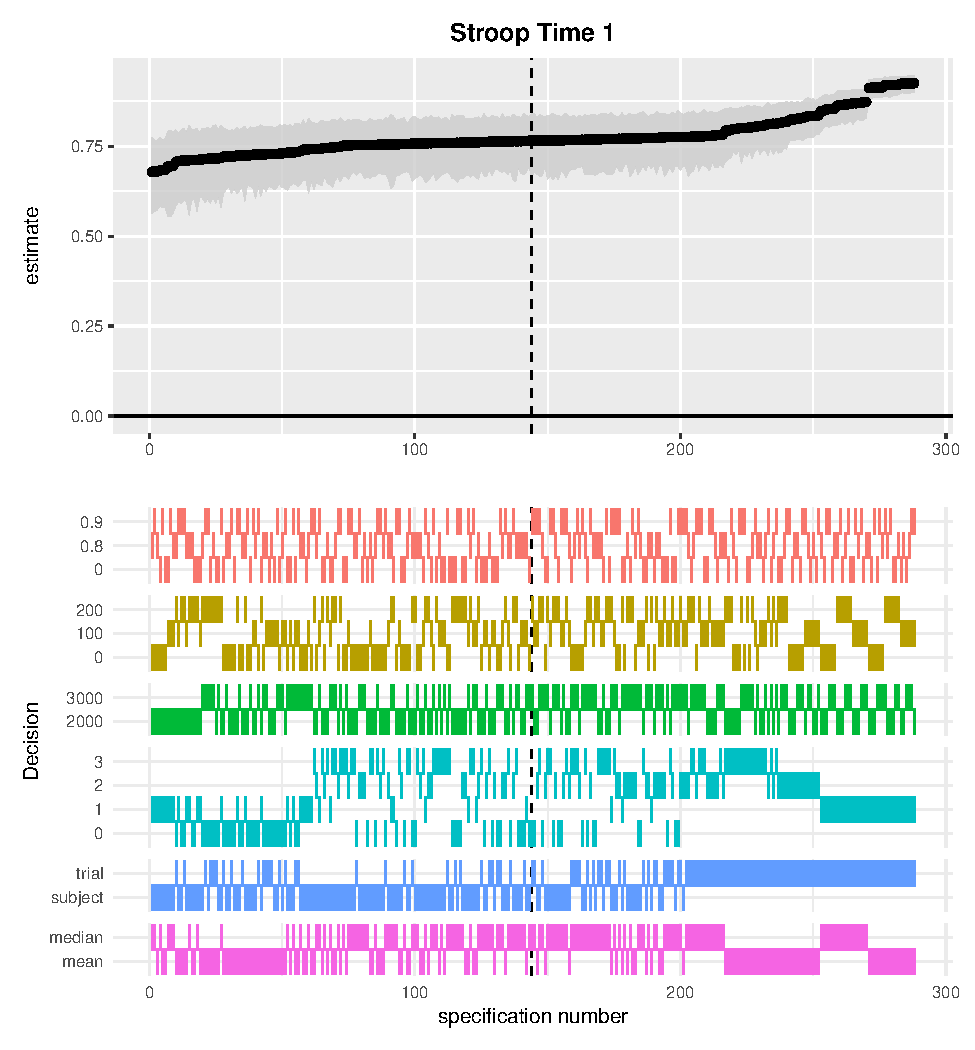
\includegraphics{Reliability_Multiverse_files/figure-latex/unnamed-chunk-5-1.pdf}
\caption{\label{fig:unnamed-chunk-5}Internal consistency reliability multiverse for Stroop RT cost at time 1}
\end{figure}

\newpage

\hypertarget{stroop-time-2-internal-consistency}{%
\subsubsection{Stroop Time 2: Internal Consistency}\label{stroop-time-2-internal-consistency}}

The median reliability estimate was 0.66, 95\% CI {[}0.61,0.89{]}. Estimates ranged from 0.58 to 0.90. 25\% of the reliability estimates were \textgreater{} 0.7.

\begin{figure}
\centering
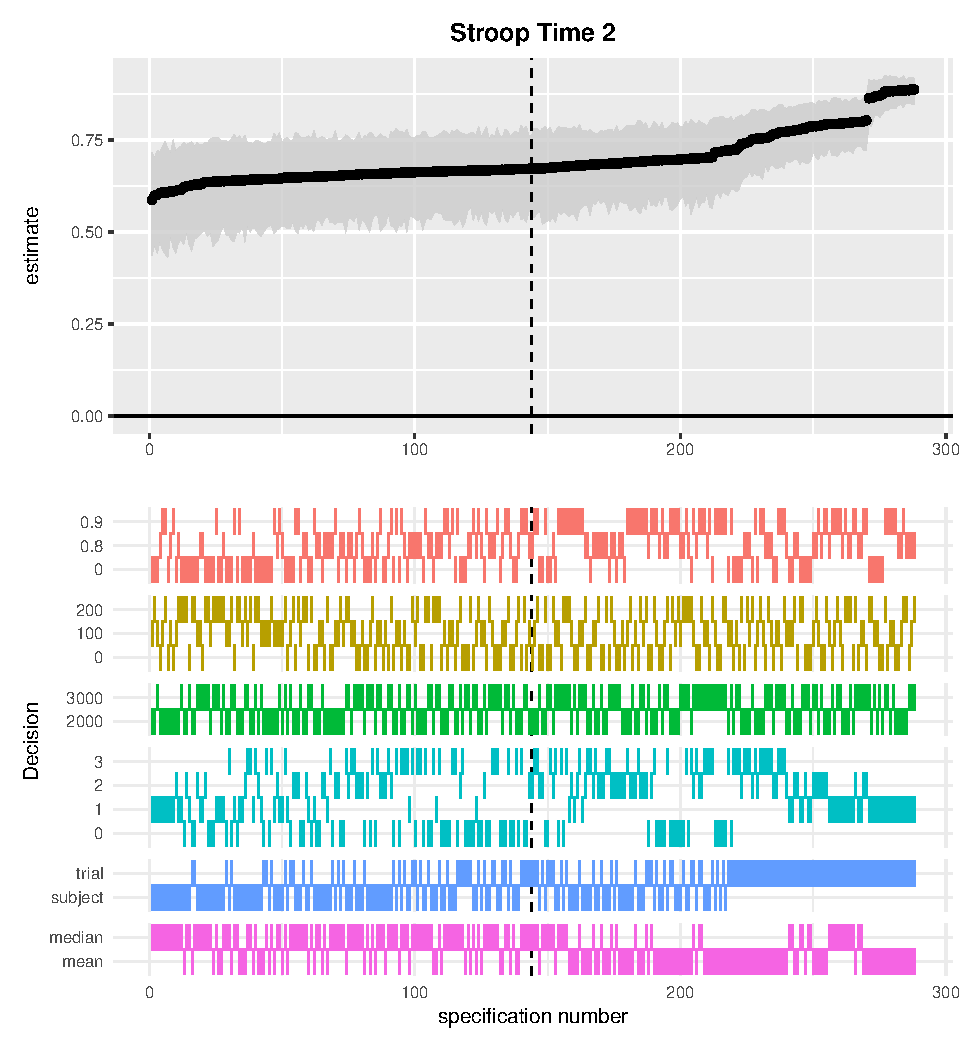
\includegraphics{Reliability_Multiverse_files/figure-latex/unnamed-chunk-6-1.pdf}
\caption{\label{fig:unnamed-chunk-6}Internal consistency reliability multiverse for Stroop RT cost at time 2}
\end{figure}

\newpage

\hypertarget{stroop-test-retest}{%
\subsubsection{Stroop: test-retest}\label{stroop-test-retest}}

The median reliability estimate was 0.56, 95\% CI {[}0.50,0.63{]}. Estimates ranged from 0.47 to 0.63. 0\% of the reliability estimates were \textgreater{} 0.7.

\begin{figure}
\centering
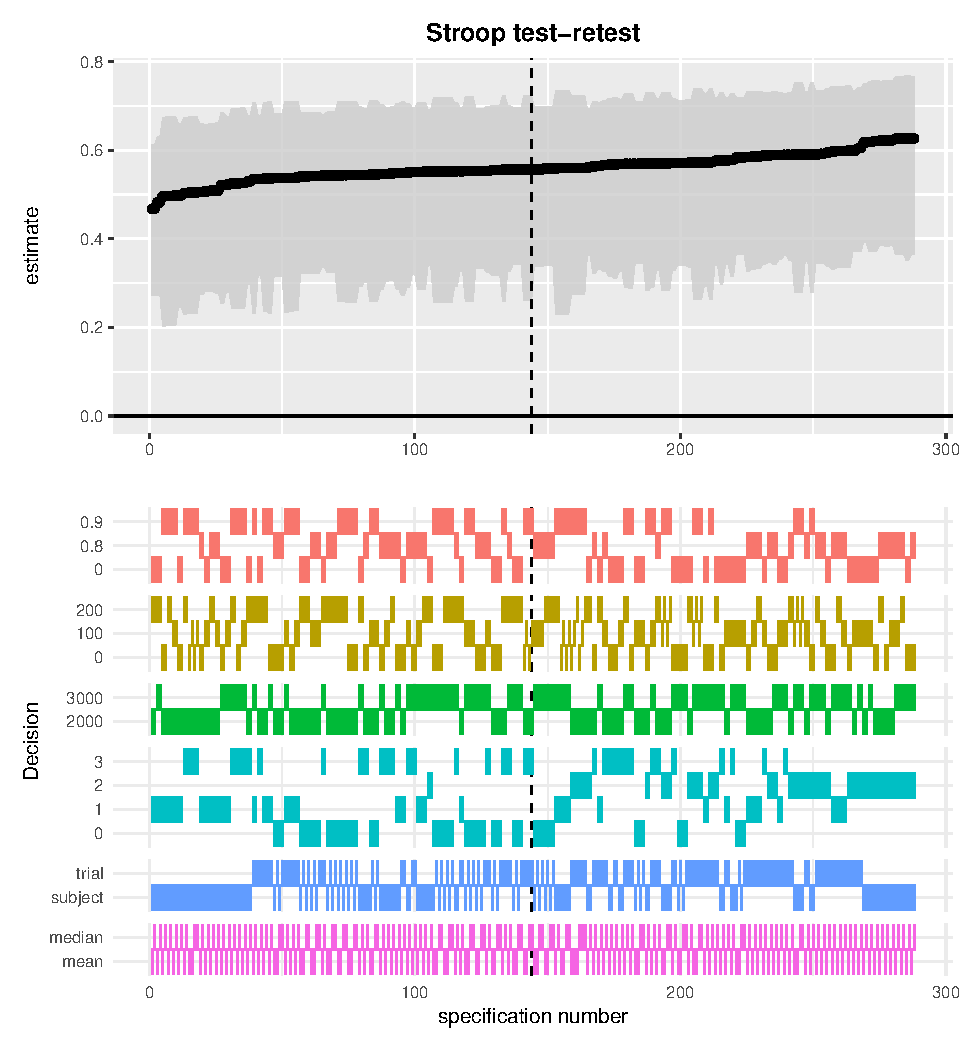
\includegraphics{Reliability_Multiverse_files/figure-latex/unnamed-chunk-7-1.pdf}
\caption{\label{fig:unnamed-chunk-7}Test-retest reliability multiverse for Stroop RT cost}
\end{figure}

\newpage

\hypertarget{flanker-time-1-internal-consistency}{%
\subsubsection{Flanker Time 1: Internal Consistency}\label{flanker-time-1-internal-consistency}}

The median reliability estimate was 0.82, 95\% CI {[}0.65,0.92{]}. Estimates ranged from 0.62 to 0.93. 93\% of the reliability estimates were \textgreater{} 0.7.

\begin{figure}
\centering
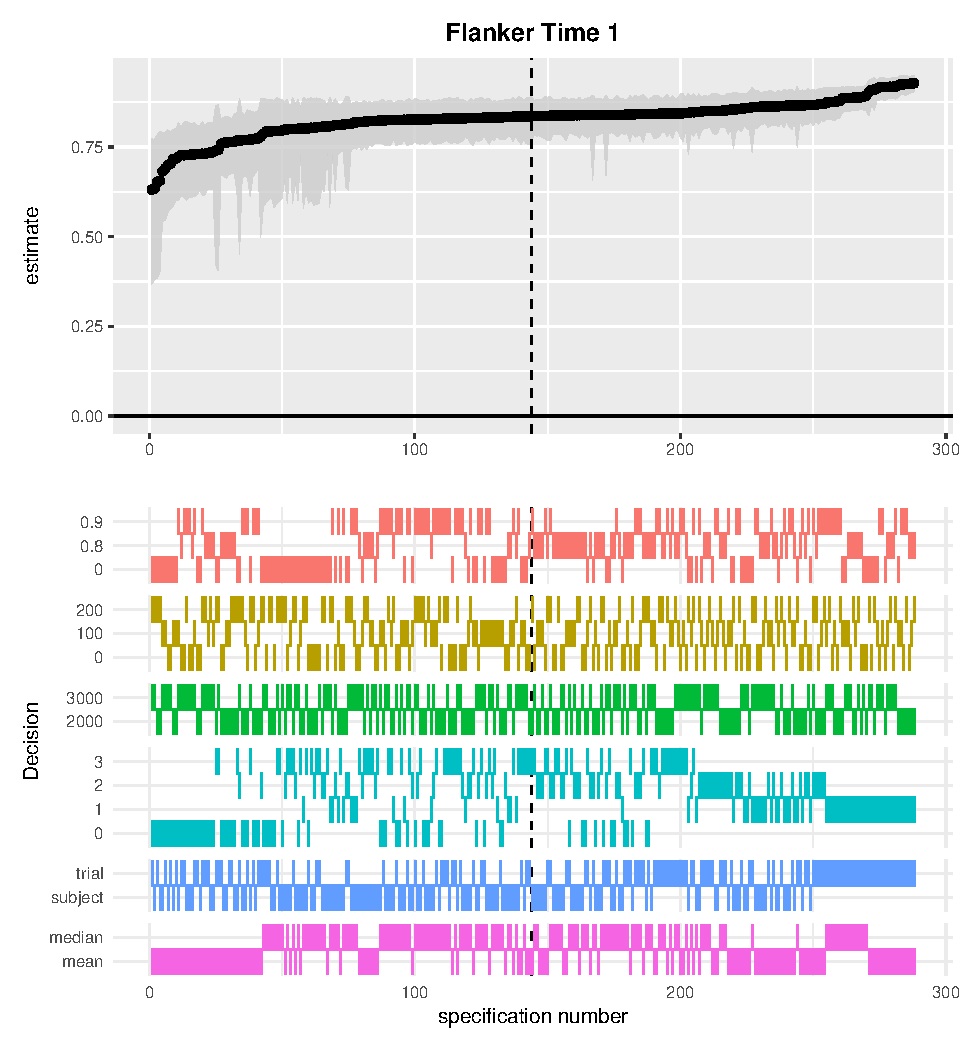
\includegraphics{Reliability_Multiverse_files/figure-latex/unnamed-chunk-8-1.pdf}
\caption{\label{fig:unnamed-chunk-8}Internal consistency reliability multiverse for Flanker RT cost at time 1}
\end{figure}

\newpage

\hypertarget{flanker-time-2-internal-consistency}{%
\subsubsection{Flanker Time 2: Internal Consistency}\label{flanker-time-2-internal-consistency}}

The median reliability estimate was 0.71, 95\% CI {[}0.63,0.91{]}. Estimates ranged from 0.59 to 0.91. 55.00\% of the reliability estimates were \textgreater{} 0.7.

\begin{figure}
\centering
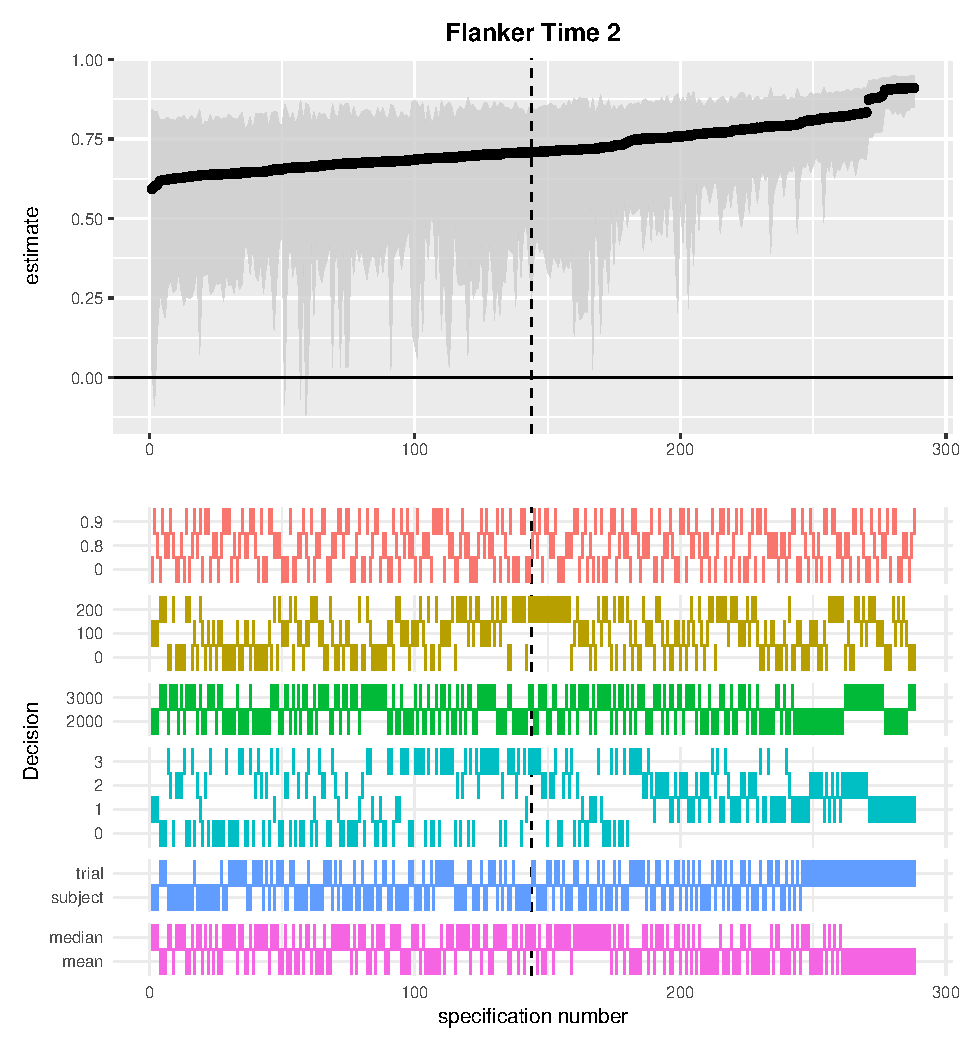
\includegraphics{Reliability_Multiverse_files/figure-latex/unnamed-chunk-9-1.pdf}
\caption{\label{fig:unnamed-chunk-9}Internal consistency reliability multiverse for Flanker RT cost at time 2}
\end{figure}

\newpage

\hypertarget{flanker-test-retest}{%
\subsubsection{Flanker: test-retest}\label{flanker-test-retest}}

The median reliability estimate was 0.55, 95\% CI {[}0.30,0.69{]}. Estimates ranged from 0.29 to 0.72. 2\% of the reliability estimates were \textgreater{} 0.7.

\begin{figure}
\centering
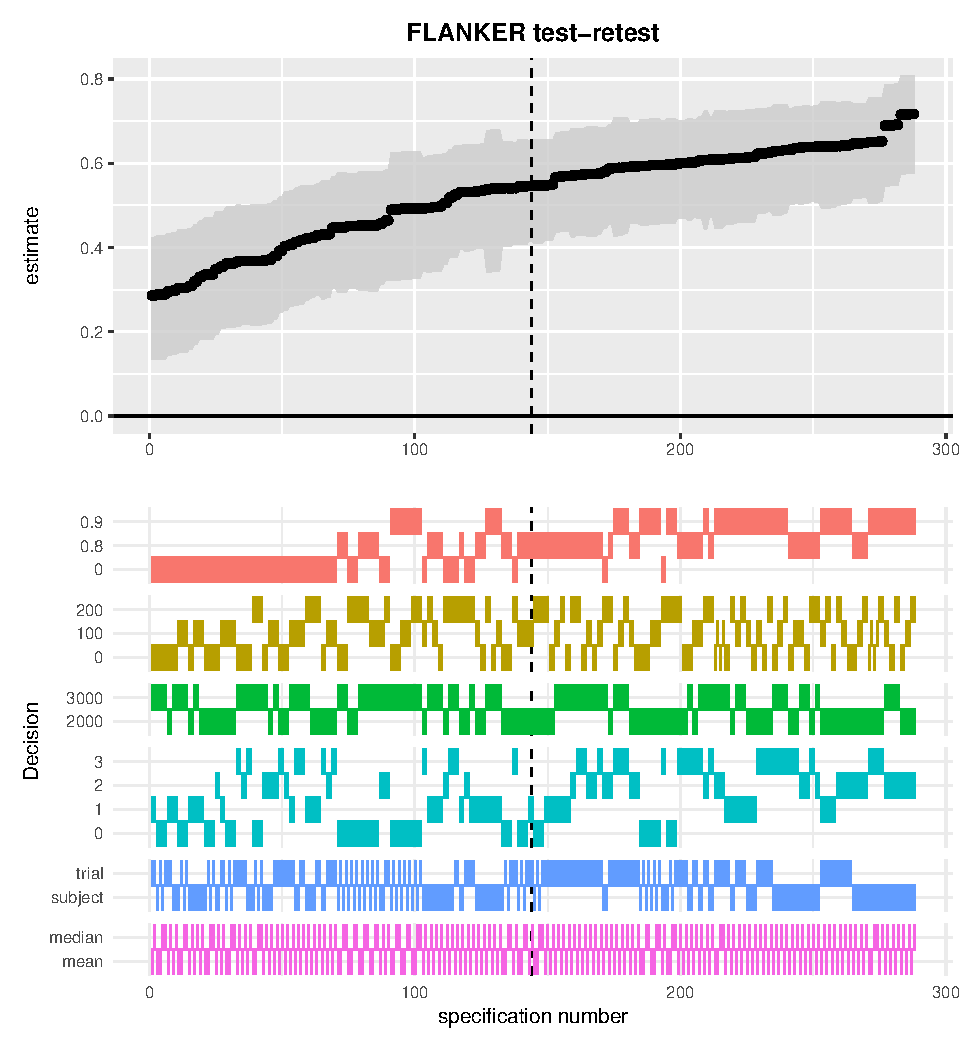
\includegraphics{Reliability_Multiverse_files/figure-latex/unnamed-chunk-10-1.pdf}
\caption{\label{fig:unnamed-chunk-10}Test-retest reliability multiverse for Flanker RT cost}
\end{figure}

\newpage

\hypertarget{overlapping-time-1-and-time-2-multiverses}{%
\subsubsection{Overlapping time 1 and time 2 multiverses}\label{overlapping-time-1-and-time-2-multiverses}}

In the next two figures I overlap the time 1 and time 2 multiverses, separately for the Stroop and Flanker data. The specifications are ordered by the reliability estimates at time 1 for each measure (Figures 1 and 3). These figures allow us to compare the patterns of reliability estimates following the same data processing decisions.

\begin{figure}
\centering
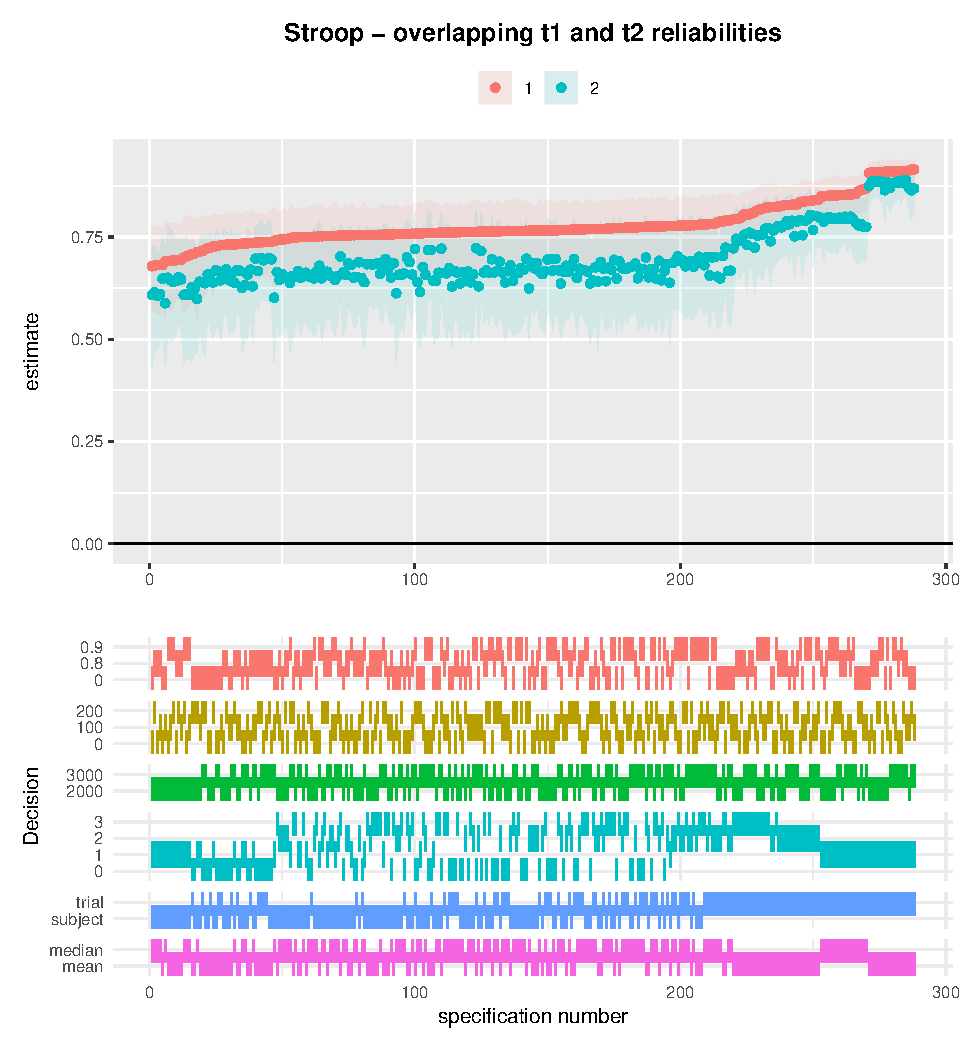
\includegraphics{Reliability_Multiverse_files/figure-latex/unnamed-chunk-11-1.pdf}
\caption{\label{fig:unnamed-chunk-11}Overlapped internal consistency reliability multiverse for Stroop RT cost at times 1 and 2}
\end{figure}

\begin{figure}
\centering
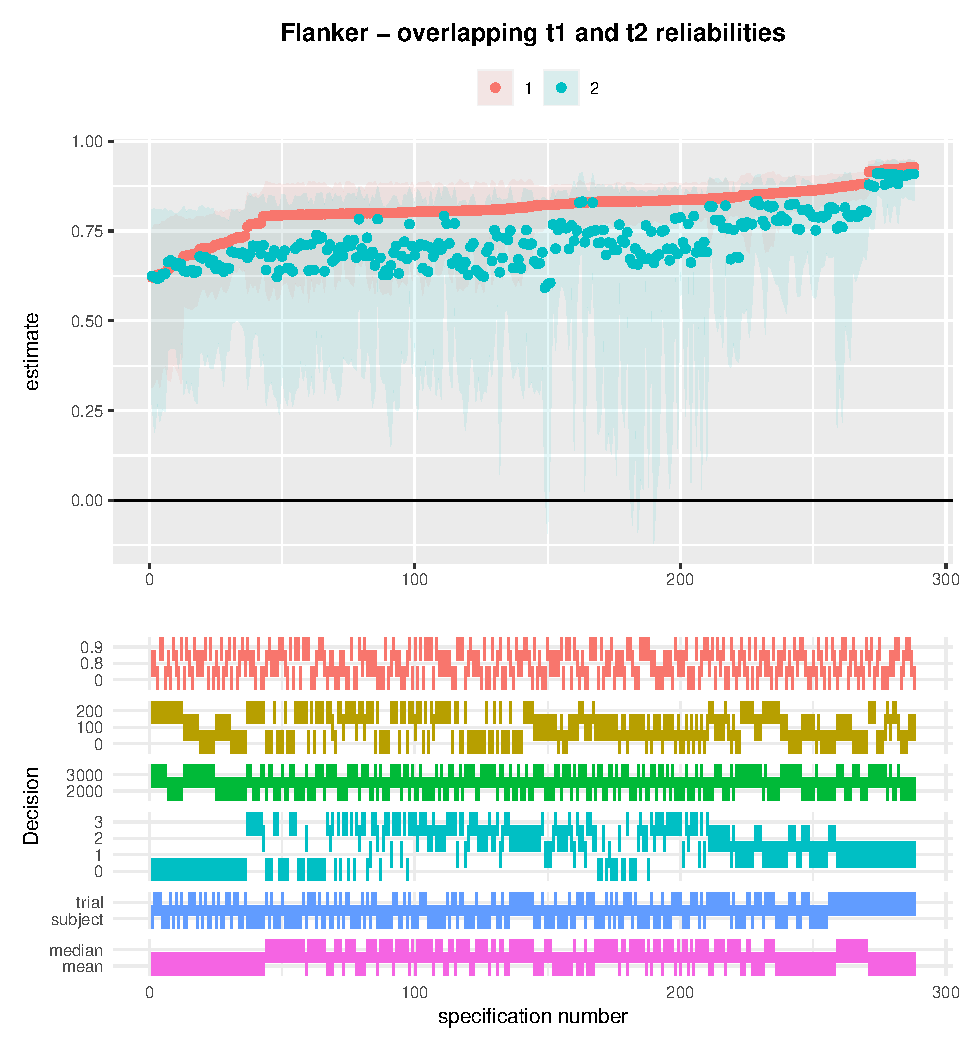
\includegraphics{Reliability_Multiverse_files/figure-latex/unnamed-chunk-12-1.pdf}
\caption{\label{fig:unnamed-chunk-12}Overlapped internal consistency reliability multiverse for Flanker RT cost at times 1 and 2}
\end{figure}

\hypertarget{dot-probe-task-1}{%
\subsection{Dot Probe Task}\label{dot-probe-task-1}}

For ease of presentation (and to reduce the total number of figures), we visualise the Dot Probe task reliability multiverses entirely as overlapping plots.

\hypertarget{angry-faces}{%
\subsubsection{Angry faces}\label{angry-faces}}

For the angry faces condition median and 95\% CIs for each wave of testing were; wave 1, -0.04, {[}95\% CI -0.17, 0.58; wave 2, 0.01, {[}95\% CI -0.21, 0.61; wave 3, 0.03, {[}95\% CI -0.08, 0.65.

\begin{figure}
\centering
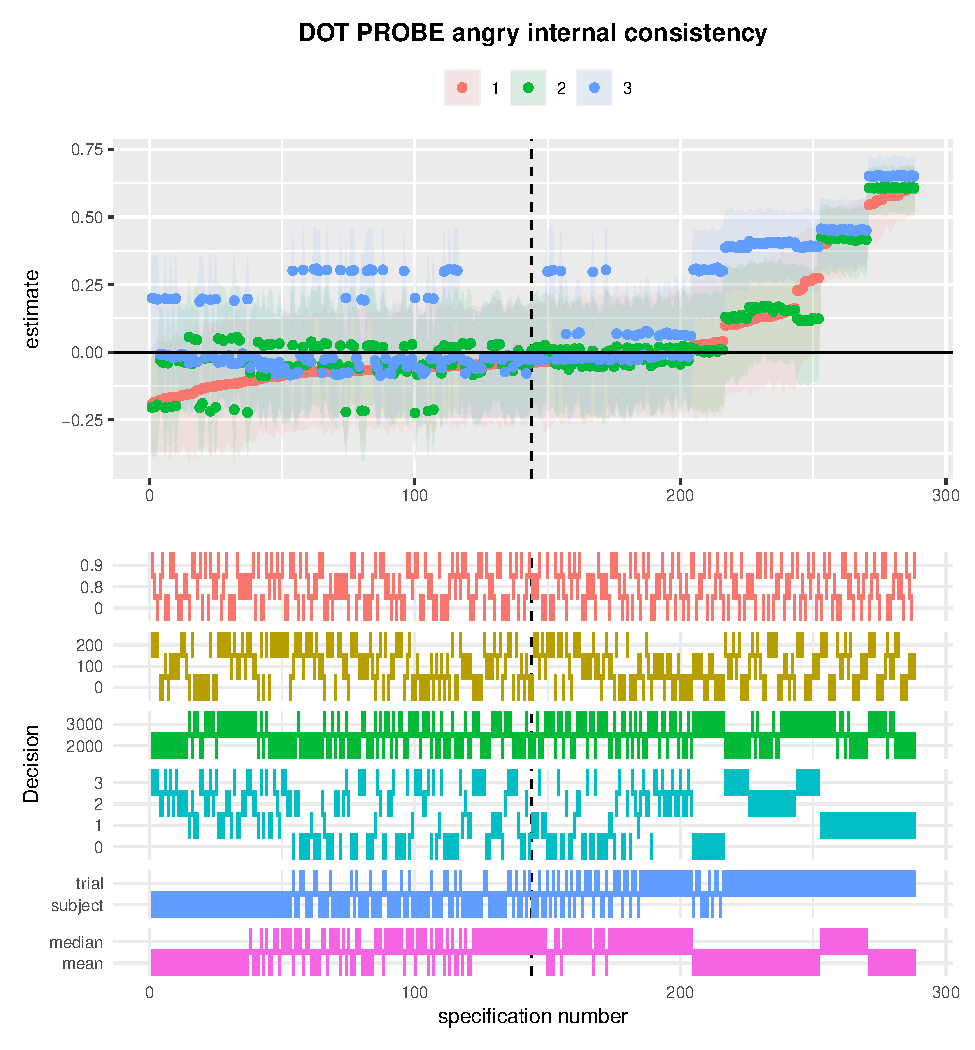
\includegraphics{Reliability_Multiverse_files/figure-latex/unnamed-chunk-13-1.pdf}
\caption{\label{fig:unnamed-chunk-13}Internal consistency reliability multiverse for Dot Probe attention bias (angry faces) at times 1, 2, and 3}
\end{figure}

\newpage

\hypertarget{happy-faces}{%
\subsubsection{Happy faces}\label{happy-faces}}

For the happy faces condition median and 95\% CIs for each wave of testing were; wave 1, -0.09, {[}95\% CI -0.19, 0.58; wave 2, -0.01, {[}95\% CI -0.10, 0.65; wave 3, 0.07, {[}95\% CI -0.04, 0.65.

\begin{figure}
\centering
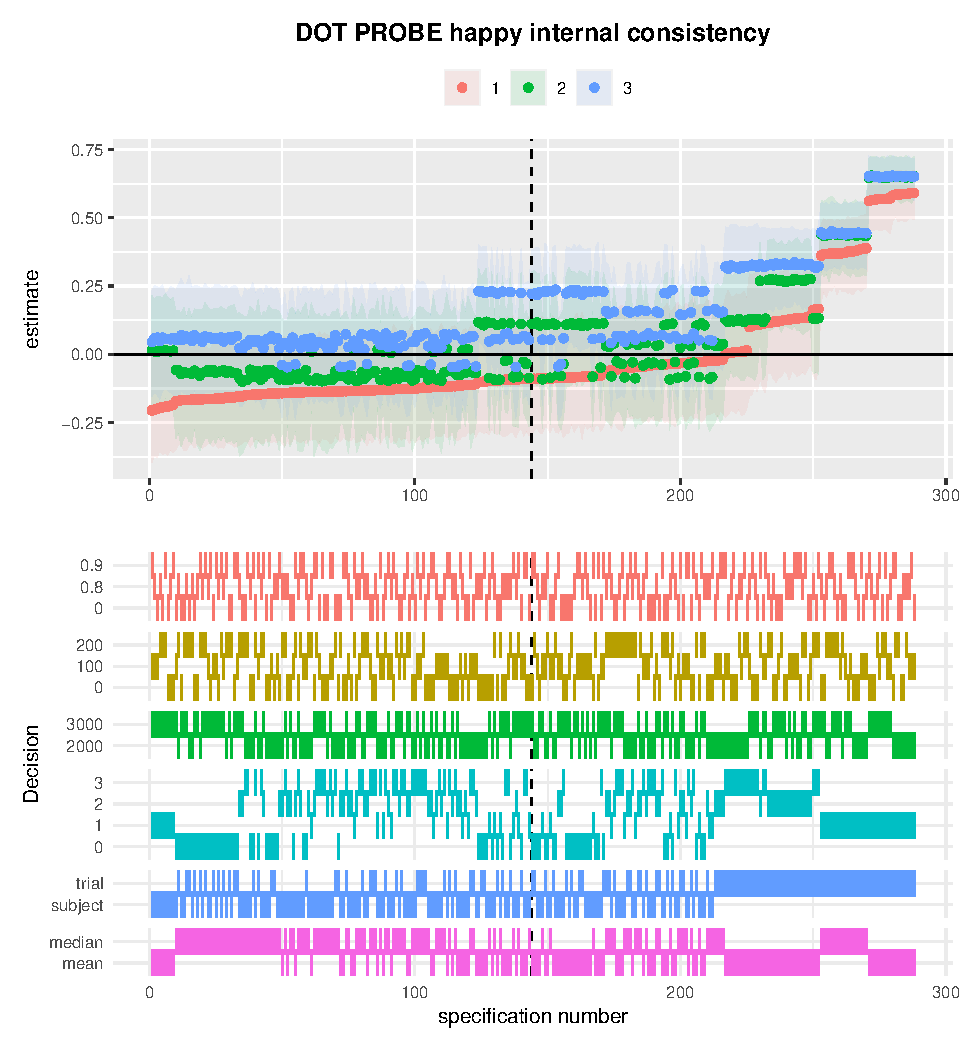
\includegraphics{Reliability_Multiverse_files/figure-latex/unnamed-chunk-14-1.pdf}
\caption{\label{fig:unnamed-chunk-14}Internal consistency reliability multiverse for Dot Probe attention bias (happy faces) at times 1, 2, and 3}
\end{figure}

\newpage

\hypertarget{pained-faces}{%
\subsubsection{Pained faces}\label{pained-faces}}

For the pained faces condition median and 95\% CIs for each wave of testing were; wave 1, 0.05, {[}95\% CI -0.26, 0.65; wave 2, -0.09, {[}95\% CI -0.18, 0.60; wave 3, 0.15, {[}95\% CI -0.08, 0.68.

\begin{figure}
\centering
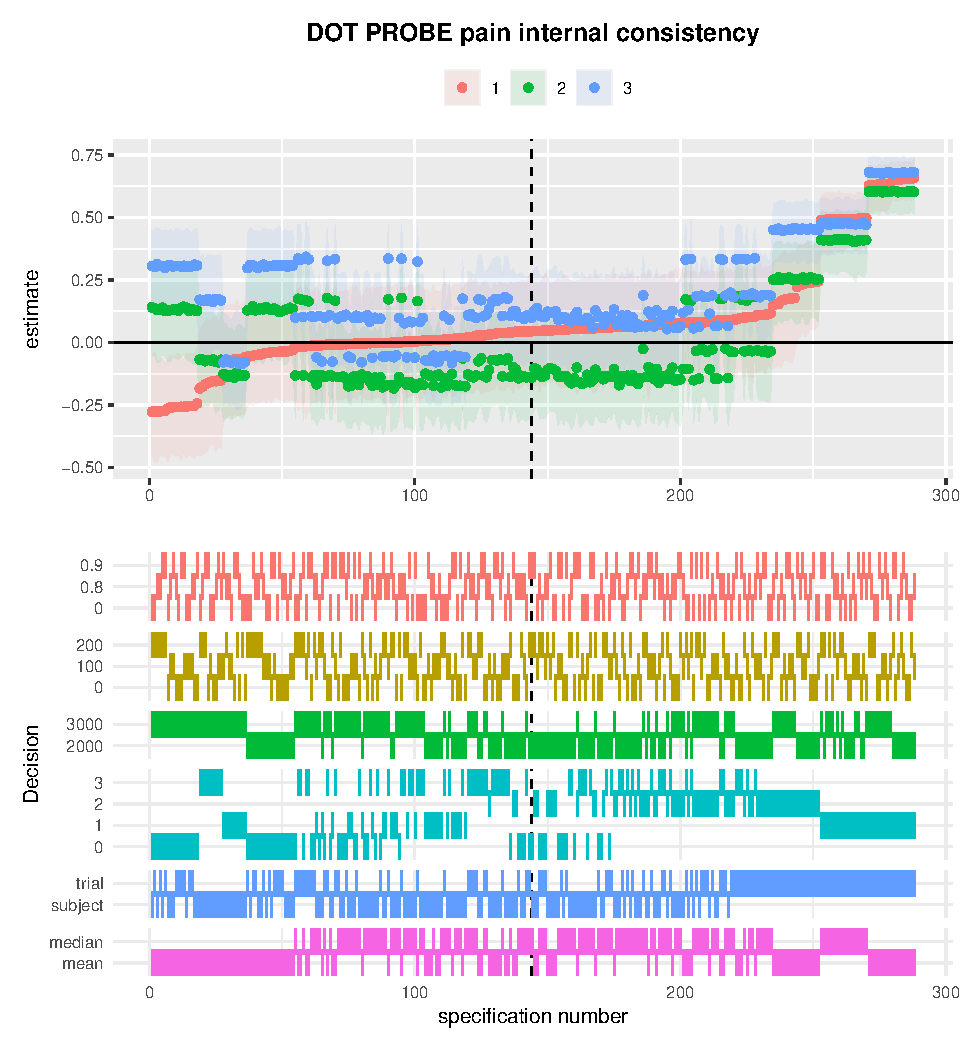
\includegraphics{Reliability_Multiverse_files/figure-latex/unnamed-chunk-15-1.pdf}
\caption{\label{fig:unnamed-chunk-15}Internal consistency reliability multiverse for Dot Probe attention bias (pain faces) at times 1, 2, and 3}
\end{figure}

\hypertarget{dot-probe-test-retest}{%
\subsubsection{Dot Probe test retest}\label{dot-probe-test-retest}}

Test retest reliability estimates (ICC2) for each condition were: angry, 0.04, 95\% CI {[}0, 0.10{]}; happy, 0, 95\% CI {[}0, 0.07{]}; pain, 0, 95\% CI {[}0, 0.01{]}

\begin{figure}
\centering
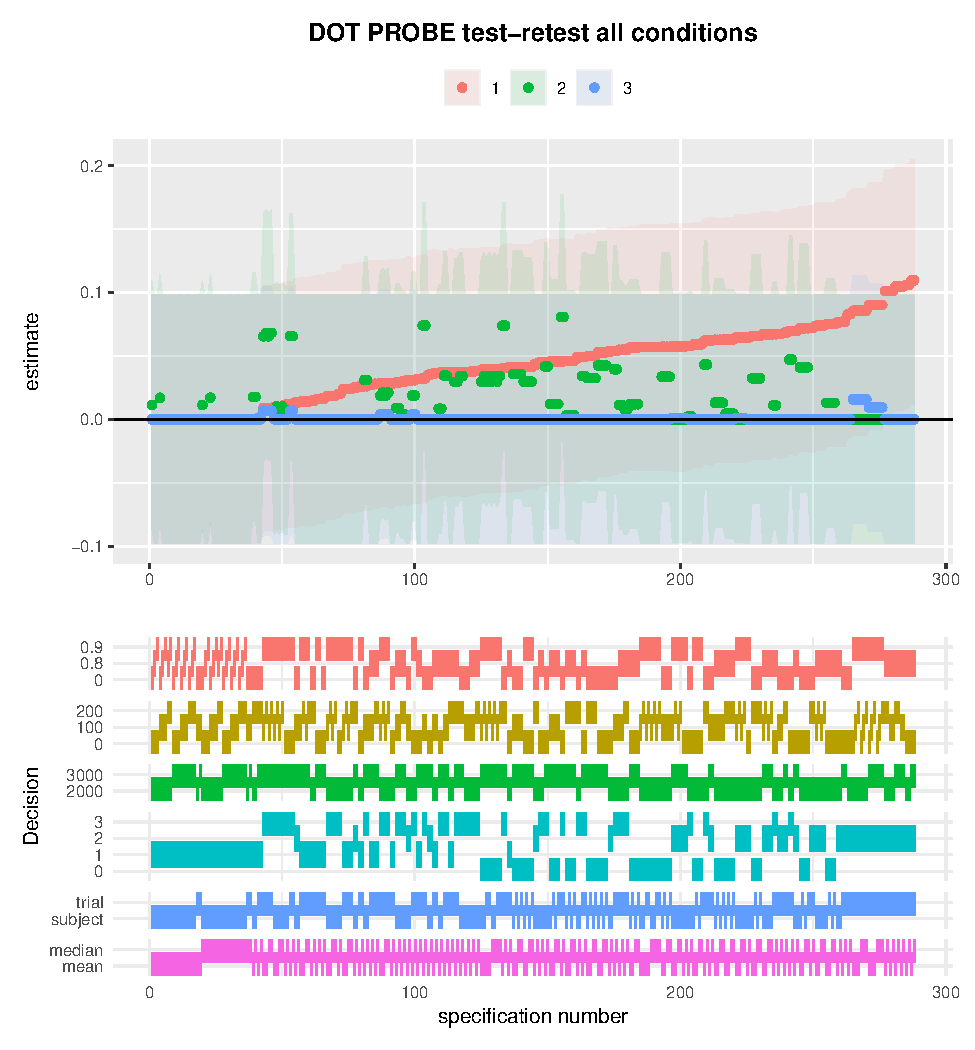
\includegraphics{Reliability_Multiverse_files/figure-latex/unnamed-chunk-16-1.pdf}
\caption{\label{fig:unnamed-chunk-16}Test-retest reliability multiverse for Dot Probe attention bias for all three conditions}
\end{figure}

\hypertarget{secondary-analyses-reliability-and-number-of-trials}{%
\subsection{Secondary analyses: reliability and number of trials}\label{secondary-analyses-reliability-and-number-of-trials}}

Increasing the number of trials typically increases reliability estimates (e.g.~Hedge et al.~2018; von Bastien et al.~2020). A visual inspection of the multiverses suggests that specifications involving the removal of more trials (i.e.~removing trials greater than 1 standard deviation from the average) leads to higher reliability estimates. Table 1 presents the Pearson correlations between the reliability estimates and the number of trials retained in each specification. For internal consistency reliability these correlations typically ran counter to expectations of reduced trials leading to reduced reliability. In most cases the association was negative - more trials removed during data processing was associated with higher reliability estimates were observed. In contrast, for most of the test-retest reliability multiverses, removal of more trials led to lower reliability estimates.

\begin{table}[tbp]

\begin{center}
\begin{threeparttable}

\caption{\label{tab:tableone}Correlations between reliability estimates and number of trials retained across specifications}

\begin{tabular}{lllrrrr}
\toprule
task & \multicolumn{1}{c}{time} & \multicolumn{1}{c}{measure} & \multicolumn{1}{c}{correlation} & \multicolumn{1}{c}{95\% CI low} & \multicolumn{1}{c}{95\% CI high} & \multicolumn{1}{c}{Difference}\\
\midrule
Stroop & 1 & splithalf & -0.39 & -0.48 & -0.28 & 0.13\\
Stroop & 2 & splithalf & -0.38 & -0.48 & -0.28 & 0.10\\
Flanker & 1 & splithalf & -0.61 & -0.68 & -0.53 & 0.12\\
Flanker & 2 & splithalf & -0.56 & -0.63 & -0.47 & 0.24\\
DPTangry & 1 & splithalf & -0.54 & -0.62 & -0.45 & -0.03\\
DPTangry & 2 & splithalf & -0.66 & -0.72 & -0.59 & -0.27\\
DPTangry & 3 & splithalf & -0.27 & -0.37 & -0.16 & -0.23\\
DPThappy & 1 & splithalf & -0.58 & -0.65 & -0.50 & -0.02\\
DPThappy & 2 & splithalf & -0.51 & -0.59 & -0.42 & -0.22\\
DPThappy & 3 & splithalf & -0.42 & -0.51 & -0.32 & -0.23\\
DPTpain & 1 & splithalf & -0.59 & -0.66 & -0.51 & -0.06\\
DPTpain & 2 & splithalf & -0.39 & -0.48 & -0.29 & -0.27\\
DPTpain & 3 & splithalf & -0.15 & -0.26 & -0.03 & -0.20\\
Stroop &  & ICC & 0.37 & 0.26 & 0.46 & 0.08\\
Flanker &  & ICC & -0.59 & -0.66 & -0.51 & 0.11\\
DPTangry &  & ICC & 0.61 & 0.54 & 0.68 & 0.04\\
DPThappy &  & ICC & 0.42 & 0.32 & 0.51 & -0.01\\
DPTpain &  & ICC & -0.01 & -0.12 & 0.11 & 0.00\\
\bottomrule
\end{tabular}

\end{threeparttable}
\end{center}

\end{table}

To investigate this further, I reran the multiverses for Stroop and Flanker data using only the first half of trials collected for each participant. I also reran the multiverses for the Dot Probe data using only the first 20 trials for each trial type (I attempted to rerun the Dot Probe data with only 14 trials for each trial type, but this led to errors under stricter specifications where there were too few trials to run the reliability estimation). To save the reader from viewing all 18 multiverses for a second time, the code and all outputs can be found in the supplementary materials. On visual inspection of the multiverse visualisations, the overall pattern of results is similar: specifications resulting in the removal of more trials tend to result in higher reliability estimates. The final column in Table 1 presents the mean difference in reliability estimates for each of the 18 multiverses (positive values indicate higher reliability estimates with the full number of trials). For internal consistency estimates: multiverses with fewer trials had lower reliability estimates, on average, for the Stroop and Flanker tasks. But, against expectations, reliability estimates increased for the Dot Probe task when the number of trials was reduced. In contrast, almost all test-retest estimates were reduced in the reduced number of trials analyses. Figure 13 presents the difference between reliability estimates in full vs reduced trials multiverses for all 18 multiverse analyses.

\begin{figure}
\centering
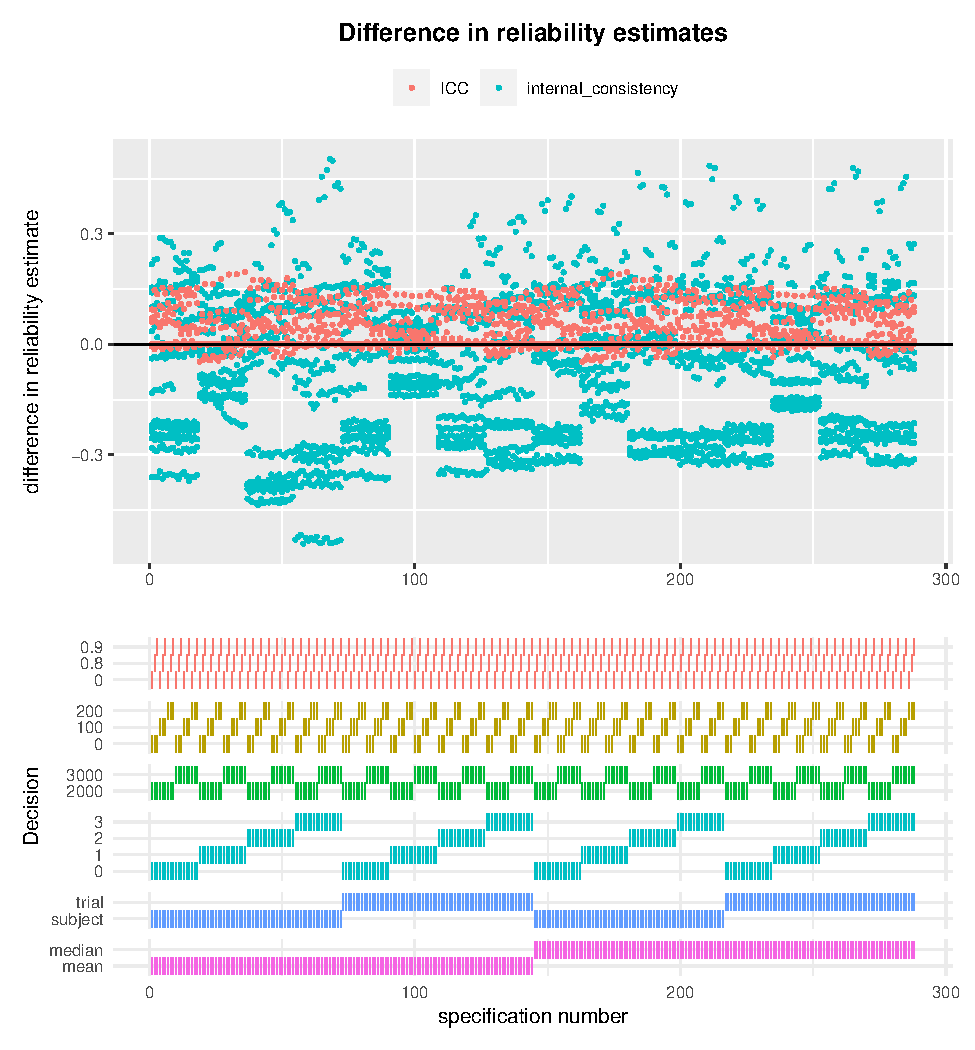
\includegraphics{Reliability_Multiverse_files/figure-latex/unnamed-chunk-18-1.pdf}
\caption{\label{fig:unnamed-chunk-18}Difference in reliability estimates from all trials to reduced trials. Note: red = angry, green = happy, blue = pained}
\end{figure}

\hypertarget{discussion}{%
\section{Discussion}\label{discussion}}

Across 18 reliability multiverse analyses, and their colourful visualisations, we explored the influence of data pre-processing specifications on measure reliability. To briefly summarise: Internal consistency reliability estimates ranged from 0.58 to 0.92 in the Stroop data, 0.59 to 0.93 in the Flanker data, and -0.28 to 0.68 in the Dot Probe data. Test-retest reliability estimates ranged from 0.47 to 0.63 in the Stroop data, 0.29 to 0.72 in the Flanker data, and 0 to 0.11 in the Dot Probe data. From the introduction we remember that reliability estimates are a product of: the sample and the population they are drawn from, the task (including any differences in implementation), and the circumstances in which the measurement was obtained, i.e.~reliability is not an inherent quality of the task itself. The first conclusion we can draw from these multiverse analyses is that data processing specifications are also an integral part of this list.

At the onset of this project, I thought it reasonable to assume that a particular feature of the data processing path might result in consistently higher (and lower) reliability estimates. The clearest indication we can take from these analyses is that there is no single set of data processing specifications, or combination of data processing decisions, that lead to improved reliability. The wide ranges of estimates are an additional cause for concern. Seemingly arbitrary data processing decisions can lead to differences of more than .3 in the reliability of a measure. These decisions are equally reasonable and logical choices, and we should not expect them to have meaningful impact on the theoretical questions being asked of the data. The reliability multiverse analyses presented here demonstrate this using data from a Stroop and a Flanker task. As well as across tasks, overlapping the time 1 and time 2 multiverses for both tasks highlights that even the same set of specifications does not lead to directly comparable internal consistency reliability estimates over time. Data processing decisions appear to be extremely important contributors to measure reliability, but their influence is unpredictable and arbitrary.

The secondary analyses give us more insight into the relationship between the number of trials retained through data processing and the resultant reliability estimates. The picture is not a simple one. Figure 13 highlights the unpredictable influence of what is essentially another multiverse specification decision -- do I remove half of trials before any other data processing? While the underlying pattern of more data reduction leading to greater reliability generally holds across tasks, within tasks fewer trials led to lower reliability on average for the Stroop and Flanker tasks (as we should expect) but not the Dot Probe. More work is needed to unravel these influences, but a take-home message may be: while administering more trials to participants is typically a good thing for reliability, there may be some benefit (in terms of reliability) of removing more trials. Though, as I discuss below, pursuit of reliability alone should not be the goal.

In the core of this discussion I raise several open questions and suggest some plausible actions that could be taken to mitigate some of the risk reliability heterogeneity poses.

\hypertarget{how-do-we-guard-against-reliability-heterogeneity}{%
\subsection{How do we guard against reliability heterogeneity?}\label{how-do-we-guard-against-reliability-heterogeneity}}

In simple bivariate analyses, we usually think low reliability will simply attenuate estimated effect sizes (e.g. Spearman, 1904). But the influence can be far less predictable (the reader may be noticing a trend of unpredictability in this paper). Low reliability can lead to elevation of effect size estimates and even reversals in direction (or examples, see Brakenhoff, Smeden, Visseren, \& Groenwold, 2018; Segerstrom \& Boggero, 2020), with the influence becoming more unpredictable in more complex models. It is therefore important to take reliability heterogeneity into account when comparing effect sizes (for several clear examples, see Cooper, Gonthier, Barch, \& Braver, 2017). It is plausible that some studies may have obtained smaller or larger effect sizes than others based, in part, on the reliability of the measurements taken. Similarly, identical observed effect sizes may represent very different `true' effect sizes, if reliability is taken into account. Recently, Wiernik and Dahlke (2020) made a strong case for correcting for measurement error in meta-analyses and provide the necessary formula and code for doing so. There are several actions we can take to begin to account for reliability heterogeneity.

\hypertarget{two-simple-recommendations.}{%
\subsubsection{Two simple recommendations.}\label{two-simple-recommendations.}}

To briefly reiterate two recommendations I and my colleagues have made previously: a) report all data processing steps taken, and b) report the reliability of measures analysed (Parsons, Kruijt, \& Fox, 2019). These recommendations will not `fix' potential psychometric issues within one's study, or reliability heterogeneity across studies. However, complete reporting of data processing will assist in the computational reproducibility of one's results. Reporting psychometric information will assist in the interpretation of results, including comparisons of effect sizes, as well as provide useful information about the utility of a task in studies of individual differences.

\hypertarget{multiverse-analyses-as-a-robustness-check}{%
\subsubsection{Multiverse analyses as a robustness check}\label{multiverse-analyses-as-a-robustness-check}}

One approach is running a multiverse across a justified set of data processing specifications (that yield the same theoretically justified construct of interest, see the below section on validity) and generating a distribution of effect sizes from the final analyses under these specifications. In principle this is the same as a sensitivity or robustness analysis, and act as a check on the reliability heterogeneity introduced by different (but equally justifiable) data processing specifications.

\hypertarget{adopt-a-modelling-approach.}{%
\subsubsection{Adopt a modelling approach.}\label{adopt-a-modelling-approach.}}

Incorporating trial level variation into our analyses with hierarchical modelling approaches (aka mixed models, multilevel models) will likely be a vital step in protecting us against reliability heterogeneity. Psychological effects are often heterogeneous across individuals (Bolger, Zee, Rossignac-Milon, \& Hassin, 2019), and factors within tasks have important effects (e.g.~stimuli differences, DeBruine \& Barr, 2019). It follows that our models should take trial-level variation into account. More than this, using models that capture the theorized data generating process, including relevant distributions (e.g.~response time distributions are typically very right skewed), likely have a better chance of capturing the process of interest in the first place. Using the Stroop and Flanker data from Hedge et al. (2018) Rouder, Kumar, and Haaf (2019; also see Rouder \& Haaf, 2018) demonstrated that hierarchical models should be used to account for error in measurement (for additional guidance on applying this modelling, see Haines, 2019). Adopting this approach has the benefit of `correcting' the effect size estimate (and standard error) for measurement error as part of the model, rather than as an additional step to aid in interpretations and effect size comparisons (a step that is often missed once reliability is deemed ``acceptable,'' assuming that reliability is estimated in the first place). Rouder and colleagues demonstrate that this is also a more effective approach than `correcting' the effect size estimate using e.g.~Spearman's correction for attenuation formula (Spearman, 1904). Yet, even better corrections cannot fully save us from measurement error.

Hierarchical measures do bring their own considerations and potential issues. Applied researchers, or those without training, may need further support to ensure the model specifications are appropriate. The model covariance structure, and appropriate priors in the case of Bayesian approaches, do have potential to introduce additional sources of bias/researcher degrees of freedom. But, given existing resources and a growing body of training materials and work in this area, it is my view that a modelling approach is likely the best next step (DeBruine \& Barr, 2021; Haines et al., 2020; Rouder, Kumar, \& Haaf, 2019; Sullivan-Toole, Haines, Dale, \& Olino, 2021). An additional benefit of these approaches is that they typically avoid much of the data pre-processing aspects discussed in this paper, and thus the reliability heterogeneity they generate.

\hypertarget{limitations-and-room-for-expansion}{%
\subsection{Limitations and room for expansion}\label{limitations-and-room-for-expansion}}

\hypertarget{a-small-number-of-tasks}{%
\subsubsection{A small number of tasks}\label{a-small-number-of-tasks}}

One limitation of this study is the focus on a small sample of tasks. It is possible that data from other tasks tend to yield more or less consistent patterns of reliability estimates across data processing specifications. Similarly, I have only examined RT costs (i.e.~a difference score between two trial types) as the outcome measure. The analyses could have examined accuracy rates, RT averages, signal detection, and a wide variety of outcome measures. It is very possible that other outcome indices would be more or less consistently reliable across the range of data processing specifications. I opted for brevity in this paper by selecting only these tasks; I welcome future work seeking to examine a wider range of tasks and outcome indices.

\hypertarget{extracting-the-influence-of-individual-decisions}{%
\subsubsection{Extracting the influence of individual decisions}\label{extracting-the-influence-of-individual-decisions}}

The analyses here do not allow for an in depth examination of the influence of specific data processing decisions. Given lack of consistency across timepoints and measures, I am not confident that robust conclusions could be drawn about a specific decision compared to another. A plausible approach to examine this is a Vibration of Effects analysis (e.g. Klau, Hoffmann, Patel, Ioannidis, \& Boulesteix, 2021) in which the variance of the final distribution of estimates can be decomposed to examine the relative influence of different categories of decisions, e.g.~model specifications and data processing decisions. Using this information, we might be able to prioritise sources of measurement heterogeneity more accurately.

\hypertarget{applicability-to-experimental-vs-correlational-analyses}{%
\subsubsection{Applicability to experimental vs correlational analyses}\label{applicability-to-experimental-vs-correlational-analyses}}

There is a paradox in measurement reliability (see Hedge, Powell, \& Sumner, 2018): Experimental effects that are highly replicable (for example, the Stroop effect) may also show low reliability. Homogeneity within groups or experimental conditions allows for larger and more robust effects; researchers can opt to develop tasks that capitalise on homogeneity. Unfortunately, reliability requires robust individual differences (and vice versa). Highly reliable measures by necessity show consistent, potentially large, individual differences and would not be suitable for group differences or experimental research. As a result, measures tend to be more appropriate for questions of a) assessing differences between groups or experimental conditions, or b) correlational or individual differences. I was primarily concerned with the use of these measures in individual differences research -- hence the focus on reliability. Yet, it would be overly simplistic to assert that the discussions in this paper do not also relate to experimental differences questions. Indeed, the data processing specifications that maximise the measure's utility in individual differences analyses can also hinder the measure's utility in experimental questions. Further research would be needed to quantify the relative influences on correlational vs experimental analyses. Yet, large fluctuations in relative between-subjects vs within-subjects variance, due to data processing, holds importance for any research question.

\hypertarget{simulation-studies}{%
\subsubsection{Simulation studies}\label{simulation-studies}}

Several valuable extensions to the current approach could be made via simulation approaches. By simulating data with a known measurement structure, we could examine variance in reliability estimates that operates purely by chance: i.e.~where no systematic differences in reliability exist across pre-processing decisions. Comparing the distributions to those observed in tasks such as those analysed here would offer insight into how severe reliability heterogeneity is introduced in ``real world'' data. These simulations are beyond the scope of this initial paper; however hold promise to detect variance and bias relative to a `true' value of reliability in the simulated data.

\hypertarget{what-about-validity}{%
\subsection{What about validity?}\label{what-about-validity}}

Others have previously demonstrated that measures are often used ad hoc or with little reported validation efforts (e.g. Flake, Pek, \& Hehman, 2017; Hussey \& Hughes, 2018). This study cannot begin to assess the influence of data processing flexibility on measure validity -- nor did this paper attempt to address this question. Reliability is only one piece of evidence needed to demonstrate the validity of a measure. Yet, it is an important piece of evidence as ``reliability provides an upper bound for validity'' (Zuo, Xu, \& Milham, 2019, p. 3). While we cannot directly conclude that flexibility in data processing influences measure validity, we should look to further research to investigate. One possibility would be to conduct a validity multiverse analysis similar to the ``Many Analysts, One Data Set'' project (Silberzahn et al., 2018). In this project, 29 teams (61 analysts total) analysed the same dataset. The teams adopted a number of different analytic approaches which resulted in a range of results. The authors concluded that, ``Uncertainty in interpreting research results is therefore not just a function of statistical power or the use of questionable research practices; it is also a function of the many reasonable decisions that researchers must make in order to conduct the research'' (page 354).

Another important validity consideration is the relationship between our data processing pipelines and the (latent) construct of interest. In questionnaire development, removing or adapting items might influence reliability. But, more importantly, will give rise to a different measure that may be more or less related to our latent construct of interest. For example, Fried (2017) found that several common depression questionnaires captured very different clusters of symptoms, which should make us question what is meant by ``depression'' in the first place when using these measures.

More relevant to task measures, to maximise reliability we might seek to develop a novel version of a task that relies on average response times, instead of a difference score between average response times. While this would yield highly reliable measures, the purpose of the difference score is to isolate the process of interest. Therefore, while we have maximized reliability, we have also influenced both the construct of interest and the validity of the measure. Perhaps this more reliable measure fails to capture the effect we intended to measure. For a more in depth discussion about balancing these theoretical, validity, and reliability considerations see von Bastian et al. (2020), Goodhew and Edwards (2019).

With respect to the data pre-processing steps taken in this paper, it could be reasonably argued that some pre-processing specifications yield different constructs of interest or could be more or less valid for the process of interest. Are we really interested in the construct including only very accurate participants and only 60\% of trials close to the average response time? In this sense, the data pre-processing decisions a researcher might adopt are certainly not arbitrary from a validity standpoint. A reasonable approach in applied work would be to select a narrower set of processing specifications that the researcher believes are theoretically similar enough that the same construct is being measured.

\hypertarget{returning-to-the-garden}{%
\subsection{Returning to the garden}\label{returning-to-the-garden}}

My intention for this project was to provide some indication about the influence of data processing pathways on the reliability of our cognitive measurements. The influence can be profound; the multiverse analyses show large differences between the highest and lowest reliability estimates. Yet, we see little consistency in the pattern of decisions leading to higher, or lower, estimates. We have the worst of both worlds: data processing decisions are largely arbitrary yet can have a large -- relatively unpredictable -- impact on the resulting reliability estimates. Briefly returning to the garden of forking paths metaphor; I imagined that this project would help illuminate the point in which our hypothetical researcher would enter the garden, based on their data processing decisions. But, our investigation has uncovered an unfortunate secret: Our researcher's forking paths are almost entirely arbitrary and interwoven. Each path diverges wildly, leading to almost anywhere in the garden. It is as if our researcher is simply spinning in dizzy circles until they stumble somewhere along the fence of reliability. I discussed several actions researchers can take collectively to help with the issue. But, by no means were these remedies to our reliability issues, nor would they directly help issues with the validity of our measurements.

Thankfully, there is a growing awareness that measurement matters (Fried \& Flake, 2018). A valuable term, Questionable Measurement Practices (QMPs), was recently added to our vernacular by Flake and Fried (2020). QMPs describe ``decisions researchers make that raise doubts about the validity of the measures used in a study, and ultimately the validity of the final conclusion'' (p.~458). I hope that QMPs and the importance of measurement become as widely discussed as the parallel idiom, `Questionable Research Practices' (QRPs). Most importantly, wider discussion of these practices should make it clear to all researchers that we make many potentially impactful decisions in the design of our measures, our data processing or cleaning, and our data analysis.

I am concerned that we sit on the precipice of a measurement crisis. The so-called replication crisis shook much of our field into widespread and ongoing reforms. Yet, much of the focus has been on improving methodological and statistical practices. This is undoubtedly worthwhile, but largely omits discussion of reliability and validity of our measurements -- despite our measurements forming the basis of any outcome or inference. This oversight feels like repairing a damaged wall at the same time as ignoring the shifting foundations under it. I hope that this paper, along other related work, highlights the issue and encourages researchers to place more emphasis on quality measurement. As a field, we can orchestrate a measurement revolution (cf.~the ``credibility revolution,'' Vazire, 2018) in which the quality and validity of our measurements is placed an order of importance above obtaining desired results. If the reader takes home a single message from this paper, please let it be ``measurement matters.''

\newpage

\hypertarget{references}{%
\section{References}\label{references}}

\begingroup
\setlength{\parindent}{-0.5in}
\setlength{\leftskip}{0.1in}

\hypertarget{refs}{}
\begin{CSLReferences}{1}{0}
\leavevmode\hypertarget{ref-R-gridExtra}{}%
Auguie, B. (2017). \emph{gridExtra: Miscellaneous functions for "grid" graphics}. Retrieved from \url{https://CRAN.R-project.org/package=gridExtra}

\leavevmode\hypertarget{ref-R-papaja}{}%
Aust, F., \& Barth, M. (2018). \emph{{papaja}: {Create} {APA} manuscripts with {R Markdown}}. Retrieved from \url{https://github.com/crsh/papaja}

\leavevmode\hypertarget{ref-von_bastian_advancing_2020}{}%
Bastian, C. C. von, Blais, C., Brewer, G. A., Gyurkovics, M., Hedge, C., Kałamała, P., \ldots{} Wiemers, E. A. (2020). \emph{Advancing the understanding of individual differences in attentional control: {Theoretical}, methodological, and analytical considerations} (preprint). PsyArXiv. \url{https://doi.org/10.31234/osf.io/x3b9k}

\leavevmode\hypertarget{ref-bolger_causal_2019}{}%
Bolger, N., Zee, K. S., Rossignac-Milon, M., \& Hassin, R. R. (2019). Causal processes in psychology are heterogeneous. \emph{Journal of Experimental Psychology: General}, \emph{148}(4), 601--618. \url{https://doi.org/10.1037/xge0000558}

\leavevmode\hypertarget{ref-booth_cogbias_2019}{}%
Booth, C., Songco, A., Parsons, S., Heathcote, L. C., \& Fox, E. (2019). The {CogBIAS} longitudinal study of adolescence: {Cohort} profile and stability and change in measures across three waves. \emph{BMC Psychology}, \emph{7}(73). \url{https://doi.org/doi.org/10.1186/s40359-019-0342-8}

\leavevmode\hypertarget{ref-booth_cogbias_2017}{}%
Booth, C., Songco, A., Parsons, S., Heathcote, L., Vincent, J., Keers, R., \& Fox, E. (2017). The {CogBIAS} longitudinal study protocol: Cognitive and genetic factors influencing psychological functioning in adolescence. \emph{BMC Psychology}, \emph{5}(1). \url{https://doi.org/10.1186/s40359-017-0210-3}

\leavevmode\hypertarget{ref-brakenhoff_random_2018}{}%
Brakenhoff, T. B., Smeden, M. van, Visseren, F. L. J., \& Groenwold, R. H. H. (2018). Random measurement error: {Why} worry? {An} example of cardiovascular risk factors. \emph{PLOS ONE}, \emph{13}(2), e0192298. \url{https://doi.org/10.1371/journal.pone.0192298}

\leavevmode\hypertarget{ref-cooper_role_2017}{}%
Cooper, S. R., Gonthier, C., Barch, D. M., \& Braver, T. S. (2017). The role of psychometrics in individual differences research in cognition: {A} case study of the {AX}-{CPT}. \emph{Frontiers in Psychology}, \emph{8}(SEP), 1--16. \url{https://doi.org/10.3389/fpsyg.2017.01482}

\leavevmode\hypertarget{ref-debruine_understanding_2019}{}%
DeBruine, L., \& Barr, D. J. (2019). \emph{Understanding mixed effects models through data simulation} (preprint). PsyArXiv. \url{https://doi.org/10.31234/osf.io/xp5cy}

\leavevmode\hypertarget{ref-debruine_understanding_2021}{}%
DeBruine, L., \& Barr, D. J. (2021). Understanding {Mixed}-{Effects} {Models} {Through} {Data} {Simulation}. \emph{Advances in Methods and Practices in Psychological Science}, \emph{4}(1), 1--15. \url{https://doi.org/10.1177/2515245920965119}

\leavevmode\hypertarget{ref-flake_measurement_2020}{}%
Flake, J. K., \& Fried, E. I. (2020). Measurement {Schmeasurement}: {Questionable} {Measurement} {Practices} and {How} to {Avoid} {Them}. \emph{Advances in Methods and Practices in Psychological Science}, \emph{3}(456-465), 10.

\leavevmode\hypertarget{ref-flake_construct_2017}{}%
Flake, J. K., Pek, J., \& Hehman, E. (2017). Construct {Validation} in {Social} and {Personality} {Research}: {Current} {Practice} and {Recommendations}. \emph{Social Psychological and Personality Science}, \emph{8}(4), 370--378. \url{https://doi.org/10.1177/1948550617693063}

\leavevmode\hypertarget{ref-fried_52_2017}{}%
Fried, E. I. (2017). The 52 symptoms of major depression: {Lack} of content overlap among seven common depression scales. \emph{Journal of Affective Disorders}, \emph{208}, 191--197. \url{https://doi.org/10.1016/j.jad.2016.10.019}

\leavevmode\hypertarget{ref-fried_measurement_2018}{}%
Fried, E. I., \& Flake, J. K. (2018). Measurement matters. \emph{Observer}. Retrieved from \url{https://www.psychologi\%20calscience.org/observer/measurement-matters}

\leavevmode\hypertarget{ref-gawronski_response_2011-1}{}%
Gawronski, B., Deutsch, R., \& Banse, R. (2011). Response {Interference} {Tasks} as {Indirect} {Measures} of {Automatic} {Associations}. In \emph{Cognitive methods in social psychology} (pp. 78--123). New York, NY, US: The Guilford Press.

\leavevmode\hypertarget{ref-gelman_garden_2013}{}%
Gelman, A., \& Loken, E. (2013). The garden of forking paths: {Why} multiple comparisons can be a problem, even when there is no {``fishing expedition''} or {``p-hacking''} and the research hypothesis was posited ahead of time, 17. Retrieved from \url{https://doi.org/dx.doi.org/10.1037/a0037714}

\leavevmode\hypertarget{ref-goodhew_translating_2019}{}%
Goodhew, S. C., \& Edwards, M. (2019). Translating experimental paradigms into individual-differences research: {Contributions}, challenges, and practical recommendations. \emph{Consciousness and Cognition}, \emph{69}, 14--25. \url{https://doi.org/10.1016/j.concog.2019.01.008}

\leavevmode\hypertarget{ref-haines_thinking_2019}{}%
Haines, N. (2019). Thinking generatively: {Why} do we use atheoretical statistical models to test substantive psychological theories? Retrieved from \url{http://haines-lab.com/post/thinking-generatively-why-do-we-use-atheoretical-statistical-models-to-test-substantive-psychological-theories/}

\leavevmode\hypertarget{ref-haines_theoretically_2020}{}%
Haines, N., Kvam, P. D., Irving, L. H., Smith, C., Beauchaine, T. P., Pitt, M. A., \ldots{} Turner, B. (2020). \emph{Theoretically {Informed} {Generative} {Models} {Can} {Advance} the {Psychological} and {Brain} {Sciences}: {Lessons} from the {Reliability} {Paradox}} (preprint). PsyArXiv. \url{https://doi.org/10.31234/osf.io/xr7y3}

\leavevmode\hypertarget{ref-hedge_reliability_2018}{}%
Hedge, C., Powell, G., \& Sumner, P. (2018). The reliability paradox: {Why} robust cognitive tasks do not produce reliable individual differences. \emph{Behavior Research Methods}, \emph{50}(3), 1166--1186. \url{https://doi.org/10.3758/s13428-017-0935-1}

\leavevmode\hypertarget{ref-R-purrr}{}%
Henry, L., \& Wickham, H. (2019). \emph{Purrr: Functional programming tools}. Retrieved from \url{https://CRAN.R-project.org/package=purrr}

\leavevmode\hypertarget{ref-hussey_hidden_2018}{}%
Hussey, I., \& Hughes, S. (2018). Hidden invalidity among fifteen commonly used measures in social and personality psychology. \url{https://doi.org/10.31234/osf.io/7rbfp}

\leavevmode\hypertarget{ref-jones_failed_2018-1}{}%
Jones, A., Christiansen, P., \& Field, M. (2018). Failed attempts to improve the reliability of the {Alcohol} {Visual} {Probe} task following empirical recommendations. \emph{Psychology of Addictive Behaviors}, \emph{32}(8), 922--932. \url{https://doi.org/10.31234/osf.io/4zsbm}

\leavevmode\hypertarget{ref-klau_examining_2021}{}%
Klau, S., Hoffmann, S., Patel, C. J., Ioannidis, J. P., \& Boulesteix, A.-L. (2021). Examining the robustness of observational associations to model, measurement and sampling uncertainty with the vibration of effects framework. \emph{International Journal of Epidemiology}, \emph{50}(1), 266--278. \url{https://doi.org/10.1093/ije/dyaa164}

\leavevmode\hypertarget{ref-koo_guideline_2016}{}%
Koo, T. K., \& Li, M. Y. (2016). A {Guideline} of {Selecting} and {Reporting} {Intraclass} {Correlation} {Coefficients} for {Reliability} {Research}. \emph{Journal of Chiropractic Medicine}, \emph{15}(2), 155--163. \url{https://doi.org/10.1016/j.jcm.2016.02.012}

\leavevmode\hypertarget{ref-lakens_justify_2018}{}%
Lakens, D., Adolfi, F. G., Albers, C. J., Anvari, F., Apps, M. A. J., Argamon, S. E., \ldots{} Zwaan, R. A. (2018). Justify your alpha. \emph{Nature Human Behaviour}, \emph{2}(3), 168--171. \url{https://doi.org/10.1038/s41562-018-0311-x}

\leavevmode\hypertarget{ref-leek_p_2015}{}%
Leek, J. T., \& Peng, R. D. (2015). P values are just the tip of the iceberg. \emph{Nature}, \emph{520}, 612. \url{https://doi.org/10.1038/520612a}

\leavevmode\hypertarget{ref-loken_measurement_2017}{}%
Loken, E., \& Gelman, A. (2017). Measurement error and the replication crisis. \emph{Science}, \emph{355}(6325), 584--585. \url{https://doi.org/10.1126/science.aal3618}

\leavevmode\hypertarget{ref-MacLeod1986}{}%
MacLeod, C., Mathews, A., \& Tata, P. (1986). Attentional bias in emotional disorders. \emph{Journal of Abnormal Psychology}, \emph{95}(1), 15--20. \url{https://doi.org/10.1037//0021-843X.95.1.15}

\leavevmode\hypertarget{ref-R-tibble}{}%
Müller, K., \& Wickham, H. (2019). \emph{Tibble: Simple data frames}. Retrieved from \url{https://CRAN.R-project.org/package=tibble}

\leavevmode\hypertarget{ref-orben_association_2019}{}%
Orben, A., \& Przybylski, A. K. (2019). The association between adolescent well-being and digital technology use. \emph{Nature Human Behaviour}, \emph{3}(2), 173--182. \url{https://doi.org/10.1038/s41562-018-0506-1}

\leavevmode\hypertarget{ref-R-splithalf}{}%
Parsons, S. (2019). Splithalf; robust estimates of split half reliability. Retrieved from \url{https://doi.org/10.6084/m9.figshare.5559175.v5}

\leavevmode\hypertarget{ref-parsons_splithalf_2021}{}%
Parsons, S. (2021). Splithalf: Robust estimates of split half reliability. \emph{Journal of Open Source Software}, \emph{6}(60), 3041. \url{https://doi.org/10.21105/joss.03041}

\leavevmode\hypertarget{ref-parsons_psychological_2019}{}%
Parsons, S., Kruijt, A.-W., \& Fox, E. (2019). Psychological {Science} {Needs} a {Standard} {Practice} of {Reporting} the {Reliability} of {Cognitive}-{Behavioral} {Measurements}. \emph{Advances in Methods and Practices in Psychological Science}, \emph{2}(4), 378--395. \url{https://doi.org/10.1177/2515245919879695}

\leavevmode\hypertarget{ref-R-patchwork}{}%
Pedersen, T. L. (2019). \emph{Patchwork: The composer of plots}. Retrieved from \url{https://CRAN.R-project.org/package=patchwork}

\leavevmode\hypertarget{ref-price_empirical_2015}{}%
Price, R. B., Kuckertz, J. M., Siegle, G. J., Ladouceur, C. D., Silk, J. S., Ryan, N. D., \ldots{} Amir, N. (2015). Empirical recommendations for improving the stability of the dot-probe task in clinical research. \emph{Psychological Assessment}, \emph{27}(2), 365--376. \url{https://doi.org/10.1037/pas0000036}

\leavevmode\hypertarget{ref-quintana_gps_2019}{}%
Quintana, D. S., \& Heathers, J. (2019). A {GPS} in the {Garden} of {Forking} {Paths} (with {Amy} {Orben}). Retrieved from \href{https://10.17605/OSF.IO/38KPE}{10.17605/OSF.IO/38KPE}

\leavevmode\hypertarget{ref-R-base}{}%
R Core Team. (2018). \emph{R: A language and environment for statistical computing}. Vienna, Austria: R Foundation for Statistical Computing. Retrieved from \url{https://www.R-project.org/}

\leavevmode\hypertarget{ref-R-psych}{}%
Revelle, W. (2019). \emph{Psych: Procedures for psychological, psychometric, and personality research}. Evanston, Illinois: Northwestern University. Retrieved from \url{https://CRAN.R-project.org/package=psych}

\leavevmode\hypertarget{ref-rohrer_probing_2017}{}%
Rohrer, J. M., Egloff, B., \& Schmukle, S. C. (2017). Probing {Birth}-{Order} {Effects} on {Narrow} {Traits} {Using} {Specification}-{Curve} {Analysis}. \emph{Psychological Science}, \emph{28}(12), 1821--1832. \url{https://doi.org/10.1177/0956797617723726}

\leavevmode\hypertarget{ref-rouder_psychometrics_2018}{}%
Rouder, J., \& Haaf, J. M. (2018). A {Psychometrics} of {Individual} {Differences} in {Experimental} {Tasks}. \url{https://doi.org/10.31234/osf.io/f3h2k}

\leavevmode\hypertarget{ref-rouder_why_2019}{}%
Rouder, J., Kumar, A., \& Haaf, J. M. (2019). Why {Most} {Studies} of {Individual} {Differences} {With} {Inhibition} {Tasks} {Are} {Bound} {To} {Fail}. \url{https://doi.org/10.31234/osf.io/3cjr5}

\leavevmode\hypertarget{ref-roy_stoic:_2009}{}%
Roy, S., Roy, C., Éthier-Majcher, C., Fortin, I., Belin, P., \& Gosselin, F. (2009). {STOIC}: {A} database of dynamic and static faces expressing highly recognizable emotions, 15. Retrieved from \url{http://mapageweb.umontreal.ca/gosselif/sroyetal_sub.pdf}

\leavevmode\hypertarget{ref-schmukle_unreliability_2005}{}%
Schmukle, S. C. (2005). Unreliability of the dot probe task. \emph{European Journal of Personality}, \emph{19}(7), 595--605. \url{https://doi.org/10.1002/per.554}

\leavevmode\hypertarget{ref-segerstrom_expected_2020}{}%
Segerstrom, S. C., \& Boggero, I. A. (2020). Expected {Estimation} {Errors} in {Studies} of the {Cortisol} {Awakening} {Response}: {A} {Simulation}. \emph{Psychosomatic Medicine}, \emph{82}(8), 751--756. \url{https://doi.org/10.1097/PSY.0000000000000850}

\leavevmode\hypertarget{ref-silberzahn_many_2018}{}%
Silberzahn, R., Uhlmann, E. L., Martin, D. P., Anselmi, P., Aust, F., Awtrey, E., \ldots{} Nosek, B. A. (2018). Many {Analysts}, {One} {Data} {Set}: {Making} {Transparent} {How} {Variations} in {Analytic} {Choices} {Affect} {Results}. \emph{Advances in Methods and Practices in Psychological Science}, \emph{1}(3), 337--356. \url{https://doi.org/10.1177/2515245917747646}

\leavevmode\hypertarget{ref-simmons_false-positive_2011}{}%
Simmons, J. P., Nelson, L. D., \& Simonsohn, U. (2011). False-{Positive} {Psychology}: {Undisclosed} {Flexibility} in {Data} {Collection} and {Analysis} {Allows} {Presenting} {Anything} as {Significant}. \emph{Psychological Science}, \emph{22}(11), 1359--1366. \url{https://doi.org/10.1177/0956797611417632}

\leavevmode\hypertarget{ref-simonsohn_specification_2015}{}%
Simonsohn, U., Simmons, J. P., \& Nelson, L. D. (2015). Specification {Curve}: {Descriptive} and {Inferential} {Statistics} on {All} {Reasonable} {Specifications}. \emph{SSRN Electronic Journal}. \url{https://doi.org/10.2139/ssrn.2694998}

\leavevmode\hypertarget{ref-spearman_proof_1904}{}%
Spearman, C. (1904). The {Proof} and {Measurement} of {Association} between {Two} {Things}. \emph{The American Journal of Psychology}, \emph{15}(1), 72. \url{https://doi.org/10.2307/1412159}

\leavevmode\hypertarget{ref-staugaard_reliability_2009}{}%
Staugaard, S. R. (2009). Reliability of two versions of the dot-probe task using photographic faces. \emph{Psychology Science Quarterly}, \emph{51}(3), 339--350.

\leavevmode\hypertarget{ref-steegen_increasing_2016}{}%
Steegen, S., Tuerlinckx, F., Gelman, A., \& Vanpaemel, W. (2016). Increasing {Transparency} {Through} a {Multiverse} {Analysis}. \emph{Perspectives on Psychological Science}, \emph{11}(5), 702--712. \url{https://doi.org/10.1177/1745691616658637}

\leavevmode\hypertarget{ref-sullivan-toole_enhancing_2021}{}%
Sullivan-Toole, H., Haines, N., Dale, K., \& Olino, T. M. (2021). \emph{Enhancing the {Psychometric} {Properties} of the {Iowa} {Gambling} {Task} {Using} {Full} {Generative} {Modeling}} (preprint). PsyArXiv. \url{https://doi.org/10.31234/osf.io/yxbjz}

\leavevmode\hypertarget{ref-R-Cairo}{}%
Urbanek, S., \& Horner, J. (2019). \emph{Cairo: R graphics device using cairo graphics library for creating high-quality bitmap (PNG, JPEG, TIFF), vector (PDF, SVG, PostScript) and display (X11 and Win32) output}. Retrieved from \url{https://CRAN.R-project.org/package=Cairo}

\leavevmode\hypertarget{ref-R-ggplot2}{}%
Wickham, H. (2016). \emph{ggplot2: Elegant graphics for data analysis}. Springer-Verlag New York. Retrieved from \url{https://ggplot2.tidyverse.org}

\leavevmode\hypertarget{ref-R-forcats}{}%
Wickham, H. (2019a). \emph{Forcats: Tools for working with categorical variables (factors)}. Retrieved from \url{https://CRAN.R-project.org/package=forcats}

\leavevmode\hypertarget{ref-R-stringr}{}%
Wickham, H. (2019b). \emph{Stringr: Simple, consistent wrappers for common string operations}. Retrieved from \url{https://CRAN.R-project.org/package=stringr}

\leavevmode\hypertarget{ref-R-tidyverse}{}%
Wickham, H., Averick, M., Bryan, J., Chang, W., McGowan, L. D., François, R., \ldots{} Yutani, H. (2019). Welcome to the {tidyverse}. \emph{Journal of Open Source Software}, \emph{4}(43), 1686. \url{https://doi.org/10.21105/joss.01686}

\leavevmode\hypertarget{ref-R-dplyr}{}%
Wickham, H., François, R., Henry, L., \& Müller, K. (2019). \emph{Dplyr: A grammar of data manipulation}. Retrieved from \url{https://CRAN.R-project.org/package=dplyr}

\leavevmode\hypertarget{ref-R-tidyr}{}%
Wickham, H., \& Henry, L. (2019). \emph{Tidyr: Tidy messy data}. Retrieved from \url{https://CRAN.R-project.org/package=tidyr}

\leavevmode\hypertarget{ref-R-readr}{}%
Wickham, H., Hester, J., \& Francois, R. (2018). \emph{Readr: Read rectangular text data}. Retrieved from \url{https://CRAN.R-project.org/package=readr}

\leavevmode\hypertarget{ref-wiernik_obtaining_2020}{}%
Wiernik, B. M., \& Dahlke, J. A. (2020). Obtaining {Unbiased} {Results} in {Meta}-{Analysis}: {The} {Importance} of {Correcting} for {Statistical} {Artifacts}. \emph{Advances in Methods and Practices in Psychological Science}. \url{https://doi.org/10.1177/2515245919885611}

\leavevmode\hypertarget{ref-zuo_harnessing_2019}{}%
Zuo, X.-N., Xu, T., \& Milham, M. P. (2019). Harnessing reliability for neuroscience research. \emph{Nature Human Behaviour}. \url{https://doi.org/10.1038/s41562-019-0655-x}

\end{CSLReferences}

\endgroup


\end{document}
